\documentclass[twoside]{book}

% Packages required by doxygen
\usepackage{fixltx2e}
\usepackage{calc}
\usepackage{doxygen}
\usepackage[export]{adjustbox} % also loads graphicx
\usepackage{graphicx}
\usepackage[utf8]{inputenc}
\usepackage{makeidx}
\usepackage{multicol}
\usepackage{multirow}
\PassOptionsToPackage{warn}{textcomp}
\usepackage{textcomp}
\usepackage[nointegrals]{wasysym}
\usepackage[table]{xcolor}

% Font selection
\usepackage[T1]{fontenc}
\usepackage[scaled=.90]{helvet}
\usepackage{courier}
\usepackage{amssymb}
\usepackage{sectsty}
\renewcommand{\familydefault}{\sfdefault}
\allsectionsfont{%
  \fontseries{bc}\selectfont%
  \color{darkgray}%
}
\renewcommand{\DoxyLabelFont}{%
  \fontseries{bc}\selectfont%
  \color{darkgray}%
}
\newcommand{\+}{\discretionary{\mbox{\scriptsize$\hookleftarrow$}}{}{}}

% Page & text layout
\usepackage{geometry}
\geometry{%
  a4paper,%
  top=2.5cm,%
  bottom=2.5cm,%
  left=2.5cm,%
  right=2.5cm%
}
\tolerance=750
\hfuzz=15pt
\hbadness=750
\setlength{\emergencystretch}{15pt}
\setlength{\parindent}{0cm}
\setlength{\parskip}{3ex plus 2ex minus 2ex}
\makeatletter
\renewcommand{\paragraph}{%
  \@startsection{paragraph}{4}{0ex}{-1.0ex}{1.0ex}{%
    \normalfont\normalsize\bfseries\SS@parafont%
  }%
}
\renewcommand{\subparagraph}{%
  \@startsection{subparagraph}{5}{0ex}{-1.0ex}{1.0ex}{%
    \normalfont\normalsize\bfseries\SS@subparafont%
  }%
}
\makeatother

% Headers & footers
\usepackage{fancyhdr}
\pagestyle{fancyplain}
\fancyhead[LE]{\fancyplain{}{\bfseries\thepage}}
\fancyhead[CE]{\fancyplain{}{}}
\fancyhead[RE]{\fancyplain{}{\bfseries\leftmark}}
\fancyhead[LO]{\fancyplain{}{\bfseries\rightmark}}
\fancyhead[CO]{\fancyplain{}{}}
\fancyhead[RO]{\fancyplain{}{\bfseries\thepage}}
\fancyfoot[LE]{\fancyplain{}{}}
\fancyfoot[CE]{\fancyplain{}{}}
\fancyfoot[RE]{\fancyplain{}{\bfseries\scriptsize Generated by Doxygen }}
\fancyfoot[LO]{\fancyplain{}{\bfseries\scriptsize Generated by Doxygen }}
\fancyfoot[CO]{\fancyplain{}{}}
\fancyfoot[RO]{\fancyplain{}{}}
\renewcommand{\footrulewidth}{0.4pt}
\renewcommand{\chaptermark}[1]{%
  \markboth{#1}{}%
}
\renewcommand{\sectionmark}[1]{%
  \markright{\thesection\ #1}%
}

% Indices & bibliography
\usepackage{natbib}
\usepackage[titles]{tocloft}
\setcounter{tocdepth}{3}
\setcounter{secnumdepth}{5}
\makeindex

% Hyperlinks (required, but should be loaded last)
\usepackage{ifpdf}
\ifpdf
  \usepackage[pdftex,pagebackref=true]{hyperref}
\else
  \usepackage[ps2pdf,pagebackref=true]{hyperref}
\fi
\hypersetup{%
  colorlinks=true,%
  linkcolor=blue,%
  citecolor=blue,%
  unicode%
}

% Custom commands
\newcommand{\clearemptydoublepage}{%
  \newpage{\pagestyle{empty}\cleardoublepage}%
}

\usepackage{caption}
\captionsetup{labelsep=space,justification=centering,font={bf},singlelinecheck=off,skip=4pt,position=top}

%===== C O N T E N T S =====

\begin{document}

% Titlepage & ToC
\hypersetup{pageanchor=false,
             bookmarksnumbered=true,
             pdfencoding=unicode
            }
\pagenumbering{alph}
\begin{titlepage}
\vspace*{7cm}
\begin{center}%
{\Large The\+Project }\\
\vspace*{1cm}
{\large Generated by Doxygen 1.8.14}\\
\end{center}
\end{titlepage}
\clearemptydoublepage
\pagenumbering{roman}
\tableofcontents
\clearemptydoublepage
\pagenumbering{arabic}
\hypersetup{pageanchor=true}

%--- Begin generated contents ---
\chapter{The\+Project}
\label{md__c_1_2__i_t__informatik_2__programmierung_1__m_s_v_s2017_entwicklung_1__projekte__the_project69d0b16be0821ba52b290d38ffbeccf6}
\Hypertarget{md__c_1_2__i_t__informatik_2__programmierung_1__m_s_v_s2017_entwicklung_1__projekte__the_project69d0b16be0821ba52b290d38ffbeccf6}
\input{md__c_1_2__i_t__informatik_2__programmierung_1__m_s_v_s2017_entwicklung_1__projekte__the_project69d0b16be0821ba52b290d38ffbeccf6}
\chapter{Bug List}
\label{bug}
\Hypertarget{bug}

\begin{DoxyRefList}
\item[\label{bug__bug000001}%
\Hypertarget{bug__bug000001}%
Member \mbox{\hyperlink{class_input_manager_acf3316661127cbdda5f0bd09cdc46a43}{Input\+Manager\+:\+:Is\+Key\+Down}} (Keyboard\+::\+Key key)]Triggers after a short delay ($\sim$500ms) when placed inside window loop. ~\newline
 
\end{DoxyRefList}
\chapter{Namespace Index}
\section{Namespace List}
Here is a list of all namespaces with brief descriptions\+:\begin{DoxyCompactList}
\item\contentsline{section}{\mbox{\hyperlink{namespace_utils}{Utils}} \\*Contains static functions that serve general purposes }{\pageref{namespace_utils}}{}
\end{DoxyCompactList}

\chapter{Hierarchical Index}
\section{Class Hierarchy}
This inheritance list is sorted roughly, but not completely, alphabetically\+:\begin{DoxyCompactList}
\item \contentsline{section}{Entity}{\pageref{class_entity}}{}
\begin{DoxyCompactList}
\item \contentsline{section}{Drawable\+Entity}{\pageref{class_drawable_entity}}{}
\end{DoxyCompactList}
\item \contentsline{section}{Finite\+State\+Machine}{\pageref{class_finite_state_machine}}{}
\item \contentsline{section}{Input\+Manager}{\pageref{class_input_manager}}{}
\item \contentsline{section}{State}{\pageref{class_state}}{}
\end{DoxyCompactList}

\chapter{Class Index}
\section{Class List}
Here are the classes, structs, unions and interfaces with brief descriptions\+:\begin{DoxyCompactList}
\item\contentsline{section}{\mbox{\hyperlink{class_drawable_entity}{Drawable\+Entity}} }{\pageref{class_drawable_entity}}{}
\item\contentsline{section}{\mbox{\hyperlink{class_entity}{Entity}} }{\pageref{class_entity}}{}
\item\contentsline{section}{\mbox{\hyperlink{class_finite_state_machine}{Finite\+State\+Machine}} }{\pageref{class_finite_state_machine}}{}
\item\contentsline{section}{\mbox{\hyperlink{class_input_manager}{Input\+Manager}} \\*Sollte eher Namespace sein. Klassen nur mit statischen Funktionen sind nicht sinnvoll }{\pageref{class_input_manager}}{}
\item\contentsline{section}{\mbox{\hyperlink{class_state}{State}} }{\pageref{class_state}}{}
\end{DoxyCompactList}

\chapter{File Index}
\section{File List}
Here is a list of all files with brief descriptions\+:\begin{DoxyCompactList}
\item\contentsline{section}{C\+:/2\+\_\+\+I\+T\+\_\+\+Informatik/2\+\_\+\+Programmierung/1\+\_\+\+M\+S\+V\+S2017\+Entwicklung/1\+\_\+\+Projekte/\+The\+Project/\+The\+Project/\+The\+Project/\mbox{\hyperlink{_drawable_entity_8h}{Drawable\+Entity.\+h}} }{\pageref{_drawable_entity_8h}}{}
\item\contentsline{section}{C\+:/2\+\_\+\+I\+T\+\_\+\+Informatik/2\+\_\+\+Programmierung/1\+\_\+\+M\+S\+V\+S2017\+Entwicklung/1\+\_\+\+Projekte/\+The\+Project/\+The\+Project/\+The\+Project/\mbox{\hyperlink{_entity_8h}{Entity.\+h}} }{\pageref{_entity_8h}}{}
\item\contentsline{section}{C\+:/2\+\_\+\+I\+T\+\_\+\+Informatik/2\+\_\+\+Programmierung/1\+\_\+\+M\+S\+V\+S2017\+Entwicklung/1\+\_\+\+Projekte/\+The\+Project/\+The\+Project/\+The\+Project/\mbox{\hyperlink{_finite_state_machine_8cpp}{Finite\+State\+Machine.\+cpp}} }{\pageref{_finite_state_machine_8cpp}}{}
\item\contentsline{section}{C\+:/2\+\_\+\+I\+T\+\_\+\+Informatik/2\+\_\+\+Programmierung/1\+\_\+\+M\+S\+V\+S2017\+Entwicklung/1\+\_\+\+Projekte/\+The\+Project/\+The\+Project/\+The\+Project/\mbox{\hyperlink{_finite_state_machine_8h}{Finite\+State\+Machine.\+h}} }{\pageref{_finite_state_machine_8h}}{}
\item\contentsline{section}{C\+:/2\+\_\+\+I\+T\+\_\+\+Informatik/2\+\_\+\+Programmierung/1\+\_\+\+M\+S\+V\+S2017\+Entwicklung/1\+\_\+\+Projekte/\+The\+Project/\+The\+Project/\+The\+Project/\mbox{\hyperlink{_input_manager_8cpp}{Input\+Manager.\+cpp}} }{\pageref{_input_manager_8cpp}}{}
\item\contentsline{section}{C\+:/2\+\_\+\+I\+T\+\_\+\+Informatik/2\+\_\+\+Programmierung/1\+\_\+\+M\+S\+V\+S2017\+Entwicklung/1\+\_\+\+Projekte/\+The\+Project/\+The\+Project/\+The\+Project/\mbox{\hyperlink{_input_manager_8h}{Input\+Manager.\+h}} }{\pageref{_input_manager_8h}}{}
\item\contentsline{section}{C\+:/2\+\_\+\+I\+T\+\_\+\+Informatik/2\+\_\+\+Programmierung/1\+\_\+\+M\+S\+V\+S2017\+Entwicklung/1\+\_\+\+Projekte/\+The\+Project/\+The\+Project/\+The\+Project/\mbox{\hyperlink{main_8cpp}{main.\+cpp}} }{\pageref{main_8cpp}}{}
\item\contentsline{section}{C\+:/2\+\_\+\+I\+T\+\_\+\+Informatik/2\+\_\+\+Programmierung/1\+\_\+\+M\+S\+V\+S2017\+Entwicklung/1\+\_\+\+Projekte/\+The\+Project/\+The\+Project/\+The\+Project/\mbox{\hyperlink{_state_8cpp}{State.\+cpp}} }{\pageref{_state_8cpp}}{}
\item\contentsline{section}{C\+:/2\+\_\+\+I\+T\+\_\+\+Informatik/2\+\_\+\+Programmierung/1\+\_\+\+M\+S\+V\+S2017\+Entwicklung/1\+\_\+\+Projekte/\+The\+Project/\+The\+Project/\+The\+Project/\mbox{\hyperlink{_state_8h}{State.\+h}} }{\pageref{_state_8h}}{}
\item\contentsline{section}{C\+:/2\+\_\+\+I\+T\+\_\+\+Informatik/2\+\_\+\+Programmierung/1\+\_\+\+M\+S\+V\+S2017\+Entwicklung/1\+\_\+\+Projekte/\+The\+Project/\+The\+Project/\+The\+Project/\mbox{\hyperlink{test_8cpp}{test.\+cpp}} }{\pageref{test_8cpp}}{}
\item\contentsline{section}{C\+:/2\+\_\+\+I\+T\+\_\+\+Informatik/2\+\_\+\+Programmierung/1\+\_\+\+M\+S\+V\+S2017\+Entwicklung/1\+\_\+\+Projekte/\+The\+Project/\+The\+Project/\+The\+Project/\mbox{\hyperlink{_utils_8h}{Utils.\+h}} }{\pageref{_utils_8h}}{}
\end{DoxyCompactList}

\chapter{Namespace Documentation}
\hypertarget{namespace_the_project}{}\section{The\+Project Namespace Reference}
\label{namespace_the_project}\index{The\+Project@{The\+Project}}
\subsection*{Namespaces}
\begin{DoxyCompactItemize}
\item 
 \mbox{\hyperlink{namespace_the_project_1_1_utils}{Utils}}
\begin{DoxyCompactList}\small\item\em Contains static functions that serve general purposes. \end{DoxyCompactList}\end{DoxyCompactItemize}
\subsection*{Classes}
\begin{DoxyCompactItemize}
\item 
class \mbox{\hyperlink{class_the_project_1_1_animated_sprite}{Animated\+Sprite}}
\item 
class \mbox{\hyperlink{class_the_project_1_1_drawable_entity}{Drawable\+Entity}}
\item 
class \mbox{\hyperlink{class_the_project_1_1_entity}{Entity}}
\item 
class \mbox{\hyperlink{class_the_project_1_1_finite_state_machine}{Finite\+State\+Machine}}
\item 
class \mbox{\hyperlink{class_the_project_1_1_input_manager}{Input\+Manager}}
\begin{DoxyCompactList}\small\item\em Sollte eher Namespace sein. Klassen nur mit statischen Funktionen sind nicht sinnvoll. \end{DoxyCompactList}\item 
class \mbox{\hyperlink{class_the_project_1_1_state}{State}}
\begin{DoxyCompactList}\small\item\em K�nnte abstrakt sein. \end{DoxyCompactList}\end{DoxyCompactItemize}
\subsection*{Enumerations}
\begin{DoxyCompactItemize}
\item 
enum \mbox{\hyperlink{namespace_the_project_a44ff561b5cef085c7b09b8461a14f7d9}{E\+State}} \{ \mbox{\hyperlink{namespace_the_project_a44ff561b5cef085c7b09b8461a14f7d9a5161d613c1d218eb6c84529604ec5469}{none}}, 
\mbox{\hyperlink{namespace_the_project_a44ff561b5cef085c7b09b8461a14f7d9a27171d1512649c717ea4d3c5abb9ae4c}{inventory}}, 
\mbox{\hyperlink{namespace_the_project_a44ff561b5cef085c7b09b8461a14f7d9a51951b246d8ef892ea94e5b5e40bb408}{main\+Menu}}
 \}
\begin{DoxyCompactList}\small\item\em Enum used to quickly access State objects inside std\+::map states of this Finite\+State\+Machine. \end{DoxyCompactList}\end{DoxyCompactItemize}


\subsection{Enumeration Type Documentation}
\mbox{\Hypertarget{namespace_the_project_a44ff561b5cef085c7b09b8461a14f7d9}\label{namespace_the_project_a44ff561b5cef085c7b09b8461a14f7d9}} 
\index{The\+Project@{The\+Project}!E\+State@{E\+State}}
\index{E\+State@{E\+State}!The\+Project@{The\+Project}}
\subsubsection{\texorpdfstring{E\+State}{EState}}
{\footnotesize\ttfamily enum \mbox{\hyperlink{namespace_the_project_a44ff561b5cef085c7b09b8461a14f7d9}{The\+Project\+::\+E\+State}}}



Enum used to quickly access \mbox{\hyperlink{class_the_project_1_1_state}{State}} objects inside std\+::map states of this \mbox{\hyperlink{class_the_project_1_1_finite_state_machine}{Finite\+State\+Machine}}. 

\begin{DoxyEnumFields}{Enumerator}
\raisebox{\heightof{T}}[0pt][0pt]{\index{none@{none}!The\+Project@{The\+Project}}\index{The\+Project@{The\+Project}!none@{none}}}\mbox{\Hypertarget{namespace_the_project_a44ff561b5cef085c7b09b8461a14f7d9a5161d613c1d218eb6c84529604ec5469}\label{namespace_the_project_a44ff561b5cef085c7b09b8461a14f7d9a5161d613c1d218eb6c84529604ec5469}} 
none&Represents the absence of a \mbox{\hyperlink{class_the_project_1_1_state}{State}}. \\
\hline

\raisebox{\heightof{T}}[0pt][0pt]{\index{inventory@{inventory}!The\+Project@{The\+Project}}\index{The\+Project@{The\+Project}!inventory@{inventory}}}\mbox{\Hypertarget{namespace_the_project_a44ff561b5cef085c7b09b8461a14f7d9a27171d1512649c717ea4d3c5abb9ae4c}\label{namespace_the_project_a44ff561b5cef085c7b09b8461a14f7d9a27171d1512649c717ea4d3c5abb9ae4c}} 
inventory&Represents the Inventory \mbox{\hyperlink{class_the_project_1_1_state}{State}}. \\
\hline

\raisebox{\heightof{T}}[0pt][0pt]{\index{main\+Menu@{main\+Menu}!The\+Project@{The\+Project}}\index{The\+Project@{The\+Project}!main\+Menu@{main\+Menu}}}\mbox{\Hypertarget{namespace_the_project_a44ff561b5cef085c7b09b8461a14f7d9a51951b246d8ef892ea94e5b5e40bb408}\label{namespace_the_project_a44ff561b5cef085c7b09b8461a14f7d9a51951b246d8ef892ea94e5b5e40bb408}} 
main\+Menu&Represents Main\+Menu \mbox{\hyperlink{class_the_project_1_1_state}{State}}. \\
\hline

\end{DoxyEnumFields}

\hypertarget{namespace_the_project_1_1_utils}{}\section{The\+Project\+:\+:Utils Namespace Reference}
\label{namespace_the_project_1_1_utils}\index{The\+Project\+::\+Utils@{The\+Project\+::\+Utils}}


Contains static functions that serve general purposes.  


\subsection*{Functions}
\begin{DoxyCompactItemize}
\item 
void \mbox{\hyperlink{namespace_the_project_1_1_utils_adcca61503685de20b939833929896854}{Pause\+Console}} ()
\begin{DoxyCompactList}\small\item\em Pauses the Console until Enter/\+Return is pressed. \end{DoxyCompactList}\end{DoxyCompactItemize}


\subsection{Detailed Description}
Contains static functions that serve general purposes. 

\subsection{Function Documentation}
\mbox{\Hypertarget{namespace_the_project_1_1_utils_adcca61503685de20b939833929896854}\label{namespace_the_project_1_1_utils_adcca61503685de20b939833929896854}} 
\index{The\+Project\+::\+Utils@{The\+Project\+::\+Utils}!Pause\+Console@{Pause\+Console}}
\index{Pause\+Console@{Pause\+Console}!The\+Project\+::\+Utils@{The\+Project\+::\+Utils}}
\subsubsection{\texorpdfstring{Pause\+Console()}{PauseConsole()}}
{\footnotesize\ttfamily void The\+Project\+::\+Utils\+::\+Pause\+Console (\begin{DoxyParamCaption}{ }\end{DoxyParamCaption})}



Pauses the Console until Enter/\+Return is pressed. 


\chapter{Class Documentation}
\hypertarget{class_the_project_1_1_animated_sprite}{}\section{The\+Project\+:\+:Animated\+Sprite Class Reference}
\label{class_the_project_1_1_animated_sprite}\index{The\+Project\+::\+Animated\+Sprite@{The\+Project\+::\+Animated\+Sprite}}


{\ttfamily \#include $<$Animated\+Sprite.\+h$>$}

Inheritance diagram for The\+Project\+:\+:Animated\+Sprite\+:\begin{figure}[H]
\begin{center}
\leavevmode
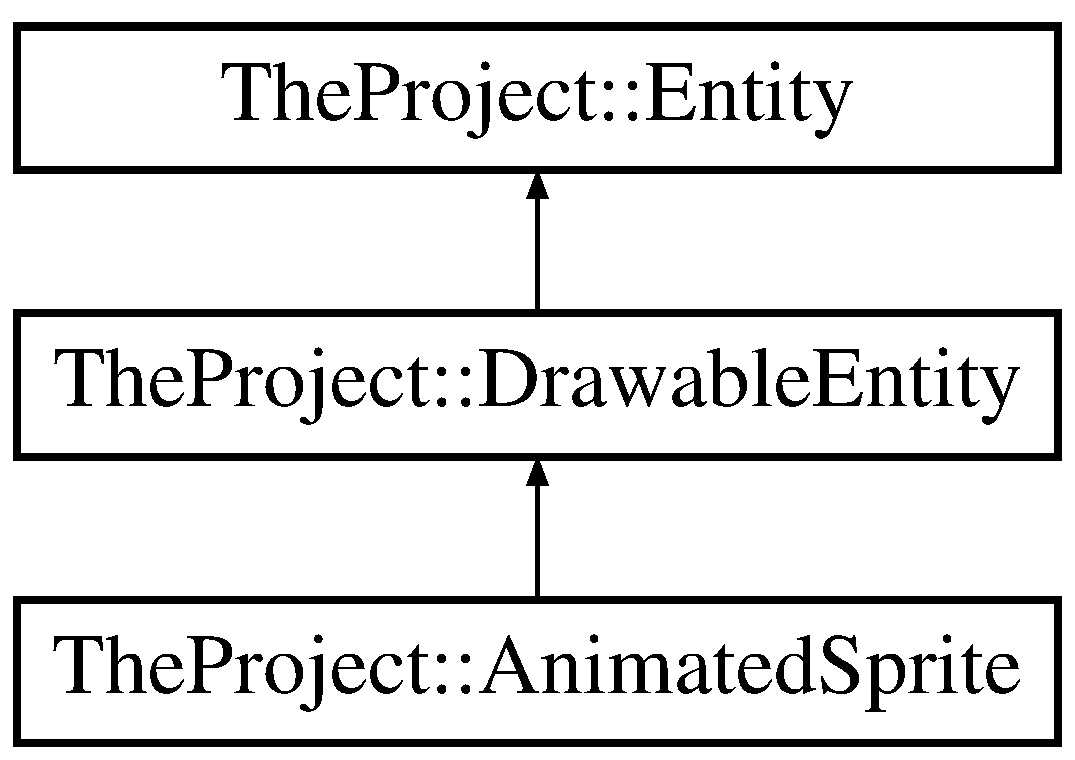
\includegraphics[height=3.000000cm]{class_the_project_1_1_animated_sprite}
\end{center}
\end{figure}
\subsection*{Public Member Functions}
\begin{DoxyCompactItemize}
\item 
\mbox{\hyperlink{class_the_project_1_1_animated_sprite_a77d348e2fe20a4ebe5b282c3c6e80b63}{Animated\+Sprite}} ()
\item 
\mbox{\hyperlink{class_the_project_1_1_animated_sprite_a7cae0bf92099bbd332f35d118d3c5d58}{$\sim$\+Animated\+Sprite}} ()
\item 
void \mbox{\hyperlink{class_the_project_1_1_animated_sprite_a25b0a4ce67cceb27c8e777443d1a8249}{update}} (float game\+Time) override
\begin{DoxyCompactList}\small\item\em Updates this \mbox{\hyperlink{class_the_project_1_1_animated_sprite}{Animated\+Sprite}}. \end{DoxyCompactList}\item 
void \mbox{\hyperlink{class_the_project_1_1_animated_sprite_ac958bbf4a60173500e5ad3bb57d268ca}{draw}} (sf\+::\+Render\+Target \&rt) const override
\begin{DoxyCompactList}\small\item\em Draws this \mbox{\hyperlink{class_the_project_1_1_animated_sprite}{Animated\+Sprite}} on the given Render\+Target. \end{DoxyCompactList}\end{DoxyCompactItemize}


\subsection{Constructor \& Destructor Documentation}
\mbox{\Hypertarget{class_the_project_1_1_animated_sprite_a77d348e2fe20a4ebe5b282c3c6e80b63}\label{class_the_project_1_1_animated_sprite_a77d348e2fe20a4ebe5b282c3c6e80b63}} 
\index{The\+Project\+::\+Animated\+Sprite@{The\+Project\+::\+Animated\+Sprite}!Animated\+Sprite@{Animated\+Sprite}}
\index{Animated\+Sprite@{Animated\+Sprite}!The\+Project\+::\+Animated\+Sprite@{The\+Project\+::\+Animated\+Sprite}}
\subsubsection{\texorpdfstring{Animated\+Sprite()}{AnimatedSprite()}}
{\footnotesize\ttfamily The\+Project\+::\+Animated\+Sprite\+::\+Animated\+Sprite (\begin{DoxyParamCaption}{ }\end{DoxyParamCaption})}

\mbox{\Hypertarget{class_the_project_1_1_animated_sprite_a7cae0bf92099bbd332f35d118d3c5d58}\label{class_the_project_1_1_animated_sprite_a7cae0bf92099bbd332f35d118d3c5d58}} 
\index{The\+Project\+::\+Animated\+Sprite@{The\+Project\+::\+Animated\+Sprite}!````~Animated\+Sprite@{$\sim$\+Animated\+Sprite}}
\index{````~Animated\+Sprite@{$\sim$\+Animated\+Sprite}!The\+Project\+::\+Animated\+Sprite@{The\+Project\+::\+Animated\+Sprite}}
\subsubsection{\texorpdfstring{$\sim$\+Animated\+Sprite()}{~AnimatedSprite()}}
{\footnotesize\ttfamily The\+Project\+::\+Animated\+Sprite\+::$\sim$\+Animated\+Sprite (\begin{DoxyParamCaption}{ }\end{DoxyParamCaption})}



\subsection{Member Function Documentation}
\mbox{\Hypertarget{class_the_project_1_1_animated_sprite_ac958bbf4a60173500e5ad3bb57d268ca}\label{class_the_project_1_1_animated_sprite_ac958bbf4a60173500e5ad3bb57d268ca}} 
\index{The\+Project\+::\+Animated\+Sprite@{The\+Project\+::\+Animated\+Sprite}!draw@{draw}}
\index{draw@{draw}!The\+Project\+::\+Animated\+Sprite@{The\+Project\+::\+Animated\+Sprite}}
\subsubsection{\texorpdfstring{draw()}{draw()}}
{\footnotesize\ttfamily void The\+Project\+::\+Animated\+Sprite\+::draw (\begin{DoxyParamCaption}\item[{sf\+::\+Render\+Target \&}]{rt }\end{DoxyParamCaption}) const\hspace{0.3cm}{\ttfamily [inline]}, {\ttfamily [override]}, {\ttfamily [virtual]}}



Draws this \mbox{\hyperlink{class_the_project_1_1_animated_sprite}{Animated\+Sprite}} on the given Render\+Target. 

\begin{DoxyAttention}{Attention}
Does inline make sense ? 
\end{DoxyAttention}

\begin{DoxyParams}{Parameters}
{\em rt} & Render\+Target that this \mbox{\hyperlink{class_the_project_1_1_animated_sprite}{Animated\+Sprite}} is drawn on \\
\hline
\end{DoxyParams}


Implements \mbox{\hyperlink{class_the_project_1_1_drawable_entity_adeb42d834f561a06b268d22f3fd354ef}{The\+Project\+::\+Drawable\+Entity}}.

\mbox{\Hypertarget{class_the_project_1_1_animated_sprite_a25b0a4ce67cceb27c8e777443d1a8249}\label{class_the_project_1_1_animated_sprite_a25b0a4ce67cceb27c8e777443d1a8249}} 
\index{The\+Project\+::\+Animated\+Sprite@{The\+Project\+::\+Animated\+Sprite}!update@{update}}
\index{update@{update}!The\+Project\+::\+Animated\+Sprite@{The\+Project\+::\+Animated\+Sprite}}
\subsubsection{\texorpdfstring{update()}{update()}}
{\footnotesize\ttfamily void The\+Project\+::\+Animated\+Sprite\+::update (\begin{DoxyParamCaption}\item[{float}]{game\+Time }\end{DoxyParamCaption})\hspace{0.3cm}{\ttfamily [override]}, {\ttfamily [virtual]}}



Updates this \mbox{\hyperlink{class_the_project_1_1_animated_sprite}{Animated\+Sprite}}. 

\begin{DoxyAttention}{Attention}
Needs additional Documentation 
\end{DoxyAttention}

\begin{DoxyParams}{Parameters}
{\em game\+Time} & Information about game\+Time \\
\hline
\end{DoxyParams}


Implements \mbox{\hyperlink{class_the_project_1_1_entity_a8ec5c42d4c918f5c98a482fb28b72da2}{The\+Project\+::\+Entity}}.



The documentation for this class was generated from the following files\+:\begin{DoxyCompactItemize}
\item 
C\+:/2\+\_\+\+I\+T\+\_\+\+Informatik/2\+\_\+\+Programmierung/1\+\_\+\+M\+S\+V\+S2017\+Entwicklung/1\+\_\+\+Projekte/\+The\+Project/\+The\+Project/\+The\+Project/\mbox{\hyperlink{_animated_sprite_8h}{Animated\+Sprite.\+h}}\item 
C\+:/2\+\_\+\+I\+T\+\_\+\+Informatik/2\+\_\+\+Programmierung/1\+\_\+\+M\+S\+V\+S2017\+Entwicklung/1\+\_\+\+Projekte/\+The\+Project/\+The\+Project/\+The\+Project/\mbox{\hyperlink{_animated_sprite_8cpp}{Animated\+Sprite.\+cpp}}\end{DoxyCompactItemize}

\hypertarget{class_the_project_1_1_drawable_entity}{}\section{The\+Project\+:\+:Drawable\+Entity Class Reference}
\label{class_the_project_1_1_drawable_entity}\index{The\+Project\+::\+Drawable\+Entity@{The\+Project\+::\+Drawable\+Entity}}


{\ttfamily \#include $<$Drawable\+Entity.\+h$>$}

Inheritance diagram for The\+Project\+:\+:Drawable\+Entity\+:\begin{figure}[H]
\begin{center}
\leavevmode
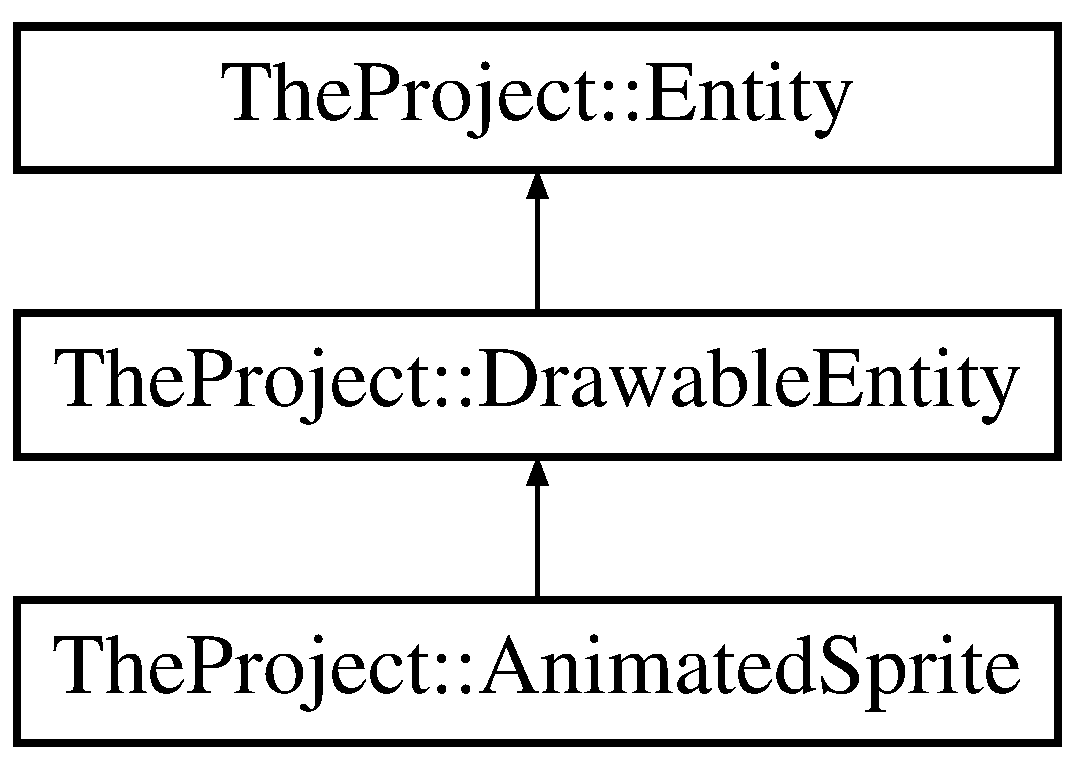
\includegraphics[height=3.000000cm]{class_the_project_1_1_drawable_entity}
\end{center}
\end{figure}
\subsection*{Public Member Functions}
\begin{DoxyCompactItemize}
\item 
virtual \mbox{\hyperlink{class_the_project_1_1_drawable_entity_a93f6204fae258f53e78d699837b1038f}{$\sim$\+Drawable\+Entity}} ()
\item 
virtual void \mbox{\hyperlink{class_the_project_1_1_drawable_entity_adeb42d834f561a06b268d22f3fd354ef}{draw}} (sf\+::\+Render\+Target \&rt) const =0
\end{DoxyCompactItemize}


\subsection{Constructor \& Destructor Documentation}
\mbox{\Hypertarget{class_the_project_1_1_drawable_entity_a93f6204fae258f53e78d699837b1038f}\label{class_the_project_1_1_drawable_entity_a93f6204fae258f53e78d699837b1038f}} 
\index{The\+Project\+::\+Drawable\+Entity@{The\+Project\+::\+Drawable\+Entity}!````~Drawable\+Entity@{$\sim$\+Drawable\+Entity}}
\index{````~Drawable\+Entity@{$\sim$\+Drawable\+Entity}!The\+Project\+::\+Drawable\+Entity@{The\+Project\+::\+Drawable\+Entity}}
\subsubsection{\texorpdfstring{$\sim$\+Drawable\+Entity()}{~DrawableEntity()}}
{\footnotesize\ttfamily virtual The\+Project\+::\+Drawable\+Entity\+::$\sim$\+Drawable\+Entity (\begin{DoxyParamCaption}{ }\end{DoxyParamCaption})\hspace{0.3cm}{\ttfamily [inline]}, {\ttfamily [virtual]}}



\subsection{Member Function Documentation}
\mbox{\Hypertarget{class_the_project_1_1_drawable_entity_adeb42d834f561a06b268d22f3fd354ef}\label{class_the_project_1_1_drawable_entity_adeb42d834f561a06b268d22f3fd354ef}} 
\index{The\+Project\+::\+Drawable\+Entity@{The\+Project\+::\+Drawable\+Entity}!draw@{draw}}
\index{draw@{draw}!The\+Project\+::\+Drawable\+Entity@{The\+Project\+::\+Drawable\+Entity}}
\subsubsection{\texorpdfstring{draw()}{draw()}}
{\footnotesize\ttfamily virtual void The\+Project\+::\+Drawable\+Entity\+::draw (\begin{DoxyParamCaption}\item[{sf\+::\+Render\+Target \&}]{rt }\end{DoxyParamCaption}) const\hspace{0.3cm}{\ttfamily [pure virtual]}}



Implemented in \mbox{\hyperlink{class_the_project_1_1_animated_sprite_ac958bbf4a60173500e5ad3bb57d268ca}{The\+Project\+::\+Animated\+Sprite}}.



The documentation for this class was generated from the following file\+:\begin{DoxyCompactItemize}
\item 
C\+:/2\+\_\+\+I\+T\+\_\+\+Informatik/2\+\_\+\+Programmierung/1\+\_\+\+M\+S\+V\+S2017\+Entwicklung/1\+\_\+\+Projekte/\+The\+Project/\+The\+Project/\+The\+Project/\mbox{\hyperlink{_drawable_entity_8h}{Drawable\+Entity.\+h}}\end{DoxyCompactItemize}

\hypertarget{class_the_project_1_1_entity}{}\section{The\+Project\+:\+:Entity Class Reference}
\label{class_the_project_1_1_entity}\index{The\+Project\+::\+Entity@{The\+Project\+::\+Entity}}


{\ttfamily \#include $<$Entity.\+h$>$}

Inheritance diagram for The\+Project\+:\+:Entity\+:\begin{figure}[H]
\begin{center}
\leavevmode
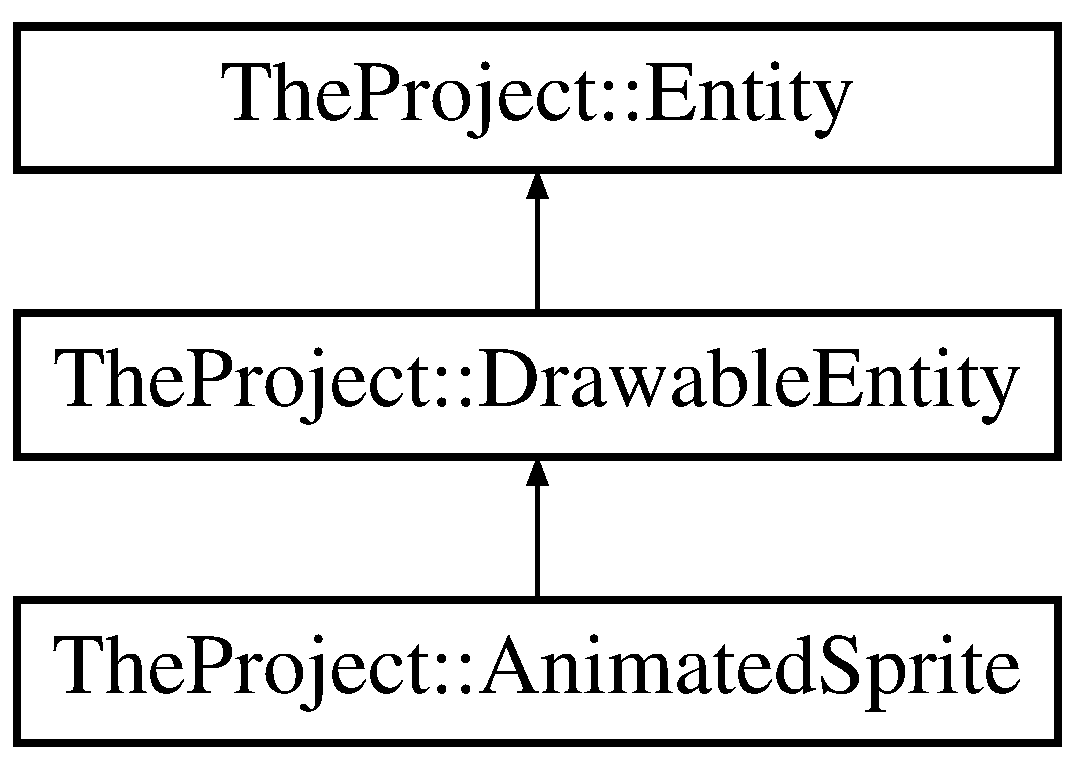
\includegraphics[height=3.000000cm]{class_the_project_1_1_entity}
\end{center}
\end{figure}
\subsection*{Public Member Functions}
\begin{DoxyCompactItemize}
\item 
virtual \mbox{\hyperlink{class_the_project_1_1_entity_aeecfd4ebad2d8d59d8945b68169add64}{$\sim$\+Entity}} ()
\item 
virtual void \mbox{\hyperlink{class_the_project_1_1_entity_a8ec5c42d4c918f5c98a482fb28b72da2}{update}} (float game\+Time)=0
\end{DoxyCompactItemize}


\subsection{Constructor \& Destructor Documentation}
\mbox{\Hypertarget{class_the_project_1_1_entity_aeecfd4ebad2d8d59d8945b68169add64}\label{class_the_project_1_1_entity_aeecfd4ebad2d8d59d8945b68169add64}} 
\index{The\+Project\+::\+Entity@{The\+Project\+::\+Entity}!````~Entity@{$\sim$\+Entity}}
\index{````~Entity@{$\sim$\+Entity}!The\+Project\+::\+Entity@{The\+Project\+::\+Entity}}
\subsubsection{\texorpdfstring{$\sim$\+Entity()}{~Entity()}}
{\footnotesize\ttfamily virtual The\+Project\+::\+Entity\+::$\sim$\+Entity (\begin{DoxyParamCaption}{ }\end{DoxyParamCaption})\hspace{0.3cm}{\ttfamily [inline]}, {\ttfamily [virtual]}}



\subsection{Member Function Documentation}
\mbox{\Hypertarget{class_the_project_1_1_entity_a8ec5c42d4c918f5c98a482fb28b72da2}\label{class_the_project_1_1_entity_a8ec5c42d4c918f5c98a482fb28b72da2}} 
\index{The\+Project\+::\+Entity@{The\+Project\+::\+Entity}!update@{update}}
\index{update@{update}!The\+Project\+::\+Entity@{The\+Project\+::\+Entity}}
\subsubsection{\texorpdfstring{update()}{update()}}
{\footnotesize\ttfamily virtual void The\+Project\+::\+Entity\+::update (\begin{DoxyParamCaption}\item[{float}]{game\+Time }\end{DoxyParamCaption})\hspace{0.3cm}{\ttfamily [pure virtual]}}



Implemented in \mbox{\hyperlink{class_the_project_1_1_animated_sprite_a25b0a4ce67cceb27c8e777443d1a8249}{The\+Project\+::\+Animated\+Sprite}}.



The documentation for this class was generated from the following file\+:\begin{DoxyCompactItemize}
\item 
C\+:/2\+\_\+\+I\+T\+\_\+\+Informatik/2\+\_\+\+Programmierung/1\+\_\+\+M\+S\+V\+S2017\+Entwicklung/1\+\_\+\+Projekte/\+The\+Project/\+The\+Project/\+The\+Project/\mbox{\hyperlink{_entity_8h}{Entity.\+h}}\end{DoxyCompactItemize}

\hypertarget{class_the_project_1_1_finite_state_machine}{}\section{The\+Project\+:\+:Finite\+State\+Machine Class Reference}
\label{class_the_project_1_1_finite_state_machine}\index{The\+Project\+::\+Finite\+State\+Machine@{The\+Project\+::\+Finite\+State\+Machine}}


{\ttfamily \#include $<$Finite\+State\+Machine.\+h$>$}

\subsection*{Public Member Functions}
\begin{DoxyCompactItemize}
\item 
\mbox{\hyperlink{class_the_project_1_1_finite_state_machine_a3328861511cf7de30f20ca54678cddbb}{Finite\+State\+Machine}} ()
\item 
\mbox{\hyperlink{class_the_project_1_1_finite_state_machine_ab719e5897533b98c1fb0ed629521de9f}{Finite\+State\+Machine}} (std\+::map$<$ \mbox{\hyperlink{namespace_the_project_a44ff561b5cef085c7b09b8461a14f7d9}{E\+State}}, \mbox{\hyperlink{class_the_project_1_1_state}{State}} $\ast$$>$ $\ast$states, \mbox{\hyperlink{namespace_the_project_a44ff561b5cef085c7b09b8461a14f7d9}{E\+State}} start\+State, \mbox{\hyperlink{namespace_the_project_a44ff561b5cef085c7b09b8461a14f7d9}{E\+State}} end\+State)
\item 
\mbox{\hyperlink{class_the_project_1_1_finite_state_machine_a5cfba82254f69404c6941e03b7d8192a}{$\sim$\+Finite\+State\+Machine}} ()
\item 
void \mbox{\hyperlink{class_the_project_1_1_finite_state_machine_adb1b07e46a5eeacdf9edb311999b0a62}{update}} (float game\+Time) const
\begin{DoxyCompactList}\small\item\em Updates the current\+State of this \mbox{\hyperlink{class_the_project_1_1_finite_state_machine}{Finite\+State\+Machine}}. \end{DoxyCompactList}\item 
void \mbox{\hyperlink{class_the_project_1_1_finite_state_machine_aeafb8ba2f752405fb1fc26c25ecbfecb}{draw}} () const
\begin{DoxyCompactList}\small\item\em Draws current\+State of this \mbox{\hyperlink{class_the_project_1_1_finite_state_machine}{Finite\+State\+Machine}}. \end{DoxyCompactList}\item 
bool \mbox{\hyperlink{class_the_project_1_1_finite_state_machine_a3c9f3d9e314c44e4845938204d8a55cd}{change}} (\mbox{\hyperlink{namespace_the_project_a44ff561b5cef085c7b09b8461a14f7d9}{E\+State}} state)
\begin{DoxyCompactList}\small\item\em If possible, changes current\+State of this \mbox{\hyperlink{class_the_project_1_1_finite_state_machine}{Finite\+State\+Machine}} to state. \end{DoxyCompactList}\item 
void \mbox{\hyperlink{class_the_project_1_1_finite_state_machine_adb1a6c6a6730d2170915a3f3bd696350}{reset}} ()
\begin{DoxyCompactList}\small\item\em Resets this \mbox{\hyperlink{class_the_project_1_1_finite_state_machine}{Finite\+State\+Machine}}(i.\+e. Restores initial \char`\"{}\+State\char`\"{}(colloquial) of this \mbox{\hyperlink{class_the_project_1_1_finite_state_machine}{Finite\+State\+Machine}}) \end{DoxyCompactList}\item 
void \mbox{\hyperlink{class_the_project_1_1_finite_state_machine_aafdc1837a9279f3509f15eff6a16828f}{terminate}} ()
\begin{DoxyCompactList}\small\item\em Terminates this \mbox{\hyperlink{class_the_project_1_1_finite_state_machine}{Finite\+State\+Machine}}(i.\+e. ????) \end{DoxyCompactList}\item 
std\+::map$<$ \mbox{\hyperlink{namespace_the_project_a44ff561b5cef085c7b09b8461a14f7d9}{E\+State}}, \mbox{\hyperlink{class_the_project_1_1_state}{State}} $\ast$ $>$ $\ast$ \mbox{\hyperlink{class_the_project_1_1_finite_state_machine_a94d221a98b4107dafe325a08642304b6}{get\+States}} () const
\begin{DoxyCompactList}\small\item\em Returns std\+::map with all States of this \mbox{\hyperlink{class_the_project_1_1_finite_state_machine}{Finite\+State\+Machine}}. \end{DoxyCompactList}\item 
\mbox{\hyperlink{namespace_the_project_a44ff561b5cef085c7b09b8461a14f7d9}{E\+State}} \mbox{\hyperlink{class_the_project_1_1_finite_state_machine_a6d6327ea03cdd29b1c03a57de907db18}{get\+Current\+State}} () const
\begin{DoxyCompactList}\small\item\em Returns E\+State current\+State of this \mbox{\hyperlink{class_the_project_1_1_finite_state_machine}{Finite\+State\+Machine}}. \end{DoxyCompactList}\item 
\mbox{\hyperlink{namespace_the_project_a44ff561b5cef085c7b09b8461a14f7d9}{E\+State}} \mbox{\hyperlink{class_the_project_1_1_finite_state_machine_aed525239e7dd0b3dc26a07e3766d8c11}{get\+Start\+State}} () const
\begin{DoxyCompactList}\small\item\em Returns E\+State start\+State of this \mbox{\hyperlink{class_the_project_1_1_finite_state_machine}{Finite\+State\+Machine}}. \end{DoxyCompactList}\item 
\mbox{\hyperlink{namespace_the_project_a44ff561b5cef085c7b09b8461a14f7d9}{E\+State}} \mbox{\hyperlink{class_the_project_1_1_finite_state_machine_ad67f02240858c7b21e499c3ed84da376}{get\+End\+State}} () const
\begin{DoxyCompactList}\small\item\em Returns E\+State end\+State of this \mbox{\hyperlink{class_the_project_1_1_finite_state_machine}{Finite\+State\+Machine}}. \end{DoxyCompactList}\end{DoxyCompactItemize}


\subsection{Constructor \& Destructor Documentation}
\mbox{\Hypertarget{class_the_project_1_1_finite_state_machine_a3328861511cf7de30f20ca54678cddbb}\label{class_the_project_1_1_finite_state_machine_a3328861511cf7de30f20ca54678cddbb}} 
\index{The\+Project\+::\+Finite\+State\+Machine@{The\+Project\+::\+Finite\+State\+Machine}!Finite\+State\+Machine@{Finite\+State\+Machine}}
\index{Finite\+State\+Machine@{Finite\+State\+Machine}!The\+Project\+::\+Finite\+State\+Machine@{The\+Project\+::\+Finite\+State\+Machine}}
\subsubsection{\texorpdfstring{Finite\+State\+Machine()}{FiniteStateMachine()}\hspace{0.1cm}{\footnotesize\ttfamily [1/2]}}
{\footnotesize\ttfamily The\+Project\+::\+Finite\+State\+Machine\+::\+Finite\+State\+Machine (\begin{DoxyParamCaption}{ }\end{DoxyParamCaption})}

\mbox{\Hypertarget{class_the_project_1_1_finite_state_machine_ab719e5897533b98c1fb0ed629521de9f}\label{class_the_project_1_1_finite_state_machine_ab719e5897533b98c1fb0ed629521de9f}} 
\index{The\+Project\+::\+Finite\+State\+Machine@{The\+Project\+::\+Finite\+State\+Machine}!Finite\+State\+Machine@{Finite\+State\+Machine}}
\index{Finite\+State\+Machine@{Finite\+State\+Machine}!The\+Project\+::\+Finite\+State\+Machine@{The\+Project\+::\+Finite\+State\+Machine}}
\subsubsection{\texorpdfstring{Finite\+State\+Machine()}{FiniteStateMachine()}\hspace{0.1cm}{\footnotesize\ttfamily [2/2]}}
{\footnotesize\ttfamily The\+Project\+::\+Finite\+State\+Machine\+::\+Finite\+State\+Machine (\begin{DoxyParamCaption}\item[{std\+::map$<$ \mbox{\hyperlink{namespace_the_project_a44ff561b5cef085c7b09b8461a14f7d9}{E\+State}}, \mbox{\hyperlink{class_the_project_1_1_state}{State}} $\ast$$>$ $\ast$}]{states,  }\item[{\mbox{\hyperlink{namespace_the_project_a44ff561b5cef085c7b09b8461a14f7d9}{E\+State}}}]{start\+State,  }\item[{\mbox{\hyperlink{namespace_the_project_a44ff561b5cef085c7b09b8461a14f7d9}{E\+State}}}]{end\+State }\end{DoxyParamCaption})}

\mbox{\Hypertarget{class_the_project_1_1_finite_state_machine_a5cfba82254f69404c6941e03b7d8192a}\label{class_the_project_1_1_finite_state_machine_a5cfba82254f69404c6941e03b7d8192a}} 
\index{The\+Project\+::\+Finite\+State\+Machine@{The\+Project\+::\+Finite\+State\+Machine}!````~Finite\+State\+Machine@{$\sim$\+Finite\+State\+Machine}}
\index{````~Finite\+State\+Machine@{$\sim$\+Finite\+State\+Machine}!The\+Project\+::\+Finite\+State\+Machine@{The\+Project\+::\+Finite\+State\+Machine}}
\subsubsection{\texorpdfstring{$\sim$\+Finite\+State\+Machine()}{~FiniteStateMachine()}}
{\footnotesize\ttfamily The\+Project\+::\+Finite\+State\+Machine\+::$\sim$\+Finite\+State\+Machine (\begin{DoxyParamCaption}{ }\end{DoxyParamCaption})}



\subsection{Member Function Documentation}
\mbox{\Hypertarget{class_the_project_1_1_finite_state_machine_a3c9f3d9e314c44e4845938204d8a55cd}\label{class_the_project_1_1_finite_state_machine_a3c9f3d9e314c44e4845938204d8a55cd}} 
\index{The\+Project\+::\+Finite\+State\+Machine@{The\+Project\+::\+Finite\+State\+Machine}!change@{change}}
\index{change@{change}!The\+Project\+::\+Finite\+State\+Machine@{The\+Project\+::\+Finite\+State\+Machine}}
\subsubsection{\texorpdfstring{change()}{change()}}
{\footnotesize\ttfamily bool The\+Project\+::\+Finite\+State\+Machine\+::change (\begin{DoxyParamCaption}\item[{\mbox{\hyperlink{namespace_the_project_a44ff561b5cef085c7b09b8461a14f7d9}{E\+State}}}]{state }\end{DoxyParamCaption})}



If possible, changes current\+State of this \mbox{\hyperlink{class_the_project_1_1_finite_state_machine}{Finite\+State\+Machine}} to state. 


\begin{DoxyParams}{Parameters}
{\em state} & \mbox{\hyperlink{class_the_project_1_1_state}{State}} that will be current\+State if \mbox{\hyperlink{class_the_project_1_1_finite_state_machine_a3c9f3d9e314c44e4845938204d8a55cd}{change()}} is successful \\
\hline
\end{DoxyParams}
\begin{DoxyReturn}{Returns}
True if change to state was successful, else false 
\end{DoxyReturn}
\mbox{\Hypertarget{class_the_project_1_1_finite_state_machine_aeafb8ba2f752405fb1fc26c25ecbfecb}\label{class_the_project_1_1_finite_state_machine_aeafb8ba2f752405fb1fc26c25ecbfecb}} 
\index{The\+Project\+::\+Finite\+State\+Machine@{The\+Project\+::\+Finite\+State\+Machine}!draw@{draw}}
\index{draw@{draw}!The\+Project\+::\+Finite\+State\+Machine@{The\+Project\+::\+Finite\+State\+Machine}}
\subsubsection{\texorpdfstring{draw()}{draw()}}
{\footnotesize\ttfamily void The\+Project\+::\+Finite\+State\+Machine\+::draw (\begin{DoxyParamCaption}{ }\end{DoxyParamCaption}) const}



Draws current\+State of this \mbox{\hyperlink{class_the_project_1_1_finite_state_machine}{Finite\+State\+Machine}}. 

\mbox{\Hypertarget{class_the_project_1_1_finite_state_machine_a6d6327ea03cdd29b1c03a57de907db18}\label{class_the_project_1_1_finite_state_machine_a6d6327ea03cdd29b1c03a57de907db18}} 
\index{The\+Project\+::\+Finite\+State\+Machine@{The\+Project\+::\+Finite\+State\+Machine}!get\+Current\+State@{get\+Current\+State}}
\index{get\+Current\+State@{get\+Current\+State}!The\+Project\+::\+Finite\+State\+Machine@{The\+Project\+::\+Finite\+State\+Machine}}
\subsubsection{\texorpdfstring{get\+Current\+State()}{getCurrentState()}}
{\footnotesize\ttfamily \mbox{\hyperlink{namespace_the_project_a44ff561b5cef085c7b09b8461a14f7d9}{E\+State}} The\+Project\+::\+Finite\+State\+Machine\+::get\+Current\+State (\begin{DoxyParamCaption}{ }\end{DoxyParamCaption}) const}



Returns E\+State current\+State of this \mbox{\hyperlink{class_the_project_1_1_finite_state_machine}{Finite\+State\+Machine}}. 

\begin{DoxyReturn}{Returns}
E\+State current\+State of this \mbox{\hyperlink{class_the_project_1_1_finite_state_machine}{Finite\+State\+Machine}} 
\end{DoxyReturn}
\mbox{\Hypertarget{class_the_project_1_1_finite_state_machine_ad67f02240858c7b21e499c3ed84da376}\label{class_the_project_1_1_finite_state_machine_ad67f02240858c7b21e499c3ed84da376}} 
\index{The\+Project\+::\+Finite\+State\+Machine@{The\+Project\+::\+Finite\+State\+Machine}!get\+End\+State@{get\+End\+State}}
\index{get\+End\+State@{get\+End\+State}!The\+Project\+::\+Finite\+State\+Machine@{The\+Project\+::\+Finite\+State\+Machine}}
\subsubsection{\texorpdfstring{get\+End\+State()}{getEndState()}}
{\footnotesize\ttfamily \mbox{\hyperlink{namespace_the_project_a44ff561b5cef085c7b09b8461a14f7d9}{E\+State}} The\+Project\+::\+Finite\+State\+Machine\+::get\+End\+State (\begin{DoxyParamCaption}{ }\end{DoxyParamCaption}) const}



Returns E\+State end\+State of this \mbox{\hyperlink{class_the_project_1_1_finite_state_machine}{Finite\+State\+Machine}}. 

\begin{DoxyReturn}{Returns}
E\+State end\+State of this \mbox{\hyperlink{class_the_project_1_1_finite_state_machine}{Finite\+State\+Machine}} 
\end{DoxyReturn}
\mbox{\Hypertarget{class_the_project_1_1_finite_state_machine_aed525239e7dd0b3dc26a07e3766d8c11}\label{class_the_project_1_1_finite_state_machine_aed525239e7dd0b3dc26a07e3766d8c11}} 
\index{The\+Project\+::\+Finite\+State\+Machine@{The\+Project\+::\+Finite\+State\+Machine}!get\+Start\+State@{get\+Start\+State}}
\index{get\+Start\+State@{get\+Start\+State}!The\+Project\+::\+Finite\+State\+Machine@{The\+Project\+::\+Finite\+State\+Machine}}
\subsubsection{\texorpdfstring{get\+Start\+State()}{getStartState()}}
{\footnotesize\ttfamily \mbox{\hyperlink{namespace_the_project_a44ff561b5cef085c7b09b8461a14f7d9}{E\+State}} The\+Project\+::\+Finite\+State\+Machine\+::get\+Start\+State (\begin{DoxyParamCaption}{ }\end{DoxyParamCaption}) const}



Returns E\+State start\+State of this \mbox{\hyperlink{class_the_project_1_1_finite_state_machine}{Finite\+State\+Machine}}. 

\begin{DoxyReturn}{Returns}
E\+State start\+State of this \mbox{\hyperlink{class_the_project_1_1_finite_state_machine}{Finite\+State\+Machine}} 
\end{DoxyReturn}
\mbox{\Hypertarget{class_the_project_1_1_finite_state_machine_a94d221a98b4107dafe325a08642304b6}\label{class_the_project_1_1_finite_state_machine_a94d221a98b4107dafe325a08642304b6}} 
\index{The\+Project\+::\+Finite\+State\+Machine@{The\+Project\+::\+Finite\+State\+Machine}!get\+States@{get\+States}}
\index{get\+States@{get\+States}!The\+Project\+::\+Finite\+State\+Machine@{The\+Project\+::\+Finite\+State\+Machine}}
\subsubsection{\texorpdfstring{get\+States()}{getStates()}}
{\footnotesize\ttfamily std\+::map$<$ \mbox{\hyperlink{namespace_the_project_a44ff561b5cef085c7b09b8461a14f7d9}{E\+State}}, \mbox{\hyperlink{class_the_project_1_1_state}{State}} $\ast$ $>$ $\ast$ The\+Project\+::\+Finite\+State\+Machine\+::get\+States (\begin{DoxyParamCaption}{ }\end{DoxyParamCaption}) const}



Returns std\+::map with all States of this \mbox{\hyperlink{class_the_project_1_1_finite_state_machine}{Finite\+State\+Machine}}. 

\begin{DoxyReturn}{Returns}
std\+::map with all States of this \mbox{\hyperlink{class_the_project_1_1_finite_state_machine}{Finite\+State\+Machine}} 
\end{DoxyReturn}
\mbox{\Hypertarget{class_the_project_1_1_finite_state_machine_adb1a6c6a6730d2170915a3f3bd696350}\label{class_the_project_1_1_finite_state_machine_adb1a6c6a6730d2170915a3f3bd696350}} 
\index{The\+Project\+::\+Finite\+State\+Machine@{The\+Project\+::\+Finite\+State\+Machine}!reset@{reset}}
\index{reset@{reset}!The\+Project\+::\+Finite\+State\+Machine@{The\+Project\+::\+Finite\+State\+Machine}}
\subsubsection{\texorpdfstring{reset()}{reset()}}
{\footnotesize\ttfamily void The\+Project\+::\+Finite\+State\+Machine\+::reset (\begin{DoxyParamCaption}{ }\end{DoxyParamCaption})}



Resets this \mbox{\hyperlink{class_the_project_1_1_finite_state_machine}{Finite\+State\+Machine}}(i.\+e. Restores initial \char`\"{}\+State\char`\"{}(colloquial) of this \mbox{\hyperlink{class_the_project_1_1_finite_state_machine}{Finite\+State\+Machine}}) 

\mbox{\Hypertarget{class_the_project_1_1_finite_state_machine_aafdc1837a9279f3509f15eff6a16828f}\label{class_the_project_1_1_finite_state_machine_aafdc1837a9279f3509f15eff6a16828f}} 
\index{The\+Project\+::\+Finite\+State\+Machine@{The\+Project\+::\+Finite\+State\+Machine}!terminate@{terminate}}
\index{terminate@{terminate}!The\+Project\+::\+Finite\+State\+Machine@{The\+Project\+::\+Finite\+State\+Machine}}
\subsubsection{\texorpdfstring{terminate()}{terminate()}}
{\footnotesize\ttfamily void The\+Project\+::\+Finite\+State\+Machine\+::terminate (\begin{DoxyParamCaption}{ }\end{DoxyParamCaption})}



Terminates this \mbox{\hyperlink{class_the_project_1_1_finite_state_machine}{Finite\+State\+Machine}}(i.\+e. ????) 

\mbox{\Hypertarget{class_the_project_1_1_finite_state_machine_adb1b07e46a5eeacdf9edb311999b0a62}\label{class_the_project_1_1_finite_state_machine_adb1b07e46a5eeacdf9edb311999b0a62}} 
\index{The\+Project\+::\+Finite\+State\+Machine@{The\+Project\+::\+Finite\+State\+Machine}!update@{update}}
\index{update@{update}!The\+Project\+::\+Finite\+State\+Machine@{The\+Project\+::\+Finite\+State\+Machine}}
\subsubsection{\texorpdfstring{update()}{update()}}
{\footnotesize\ttfamily void The\+Project\+::\+Finite\+State\+Machine\+::update (\begin{DoxyParamCaption}\item[{float}]{game\+Time }\end{DoxyParamCaption}) const}



Updates the current\+State of this \mbox{\hyperlink{class_the_project_1_1_finite_state_machine}{Finite\+State\+Machine}}. 


\begin{DoxyParams}{Parameters}
{\em game\+Time} & ???? Besser w�re Game\+Time Klasse mit mehreren Informationen (elapsed, etc.) \\
\hline
\end{DoxyParams}


The documentation for this class was generated from the following files\+:\begin{DoxyCompactItemize}
\item 
C\+:/2\+\_\+\+I\+T\+\_\+\+Informatik/2\+\_\+\+Programmierung/1\+\_\+\+M\+S\+V\+S2017\+Entwicklung/1\+\_\+\+Projekte/\+The\+Project/\+The\+Project/\+The\+Project/\mbox{\hyperlink{_finite_state_machine_8h}{Finite\+State\+Machine.\+h}}\item 
C\+:/2\+\_\+\+I\+T\+\_\+\+Informatik/2\+\_\+\+Programmierung/1\+\_\+\+M\+S\+V\+S2017\+Entwicklung/1\+\_\+\+Projekte/\+The\+Project/\+The\+Project/\+The\+Project/\mbox{\hyperlink{_finite_state_machine_8cpp}{Finite\+State\+Machine.\+cpp}}\end{DoxyCompactItemize}

\hypertarget{class_the_project_1_1_input_manager}{}\section{The\+Project\+:\+:Input\+Manager Class Reference}
\label{class_the_project_1_1_input_manager}\index{The\+Project\+::\+Input\+Manager@{The\+Project\+::\+Input\+Manager}}


Sollte eher Namespace sein. Klassen nur mit statischen Funktionen sind nicht sinnvoll.  




{\ttfamily \#include $<$Input\+Manager.\+h$>$}

\subsection*{Public Member Functions}
\begin{DoxyCompactItemize}
\item 
\mbox{\hyperlink{class_the_project_1_1_input_manager_a4bee47367bbc3f06230a564483577981}{Input\+Manager}} ()
\begin{DoxyCompactList}\small\item\em Constructor. \end{DoxyCompactList}\item 
\mbox{\hyperlink{class_the_project_1_1_input_manager_a706dff36758aa33b2f9057849ee74dca}{$\sim$\+Input\+Manager}} ()
\begin{DoxyCompactList}\small\item\em Destructor. \end{DoxyCompactList}\item 
void \mbox{\hyperlink{class_the_project_1_1_input_manager_a766d64cfa0d1ad4e78b42c03a32d02eb}{Update\+Current\+States}} ()
\begin{DoxyCompactList}\small\item\em Updates current Key States. Call before you\textquotesingle{}r Key-\/\+Operations. \end{DoxyCompactList}\item 
void \mbox{\hyperlink{class_the_project_1_1_input_manager_aefc6ce350e1ab78cc3aaef145c55a65a}{Update\+Previous\+States}} ()
\begin{DoxyCompactList}\small\item\em Updates previous Key States. Call after you\textquotesingle{}r Key-\/\+Operations. \end{DoxyCompactList}\item 
bool \mbox{\hyperlink{class_the_project_1_1_input_manager_aba7f889c5258aa96a7314371755a03ac}{On\+Key\+Down}} (Keyboard\+::\+Key key)
\begin{DoxyCompactList}\small\item\em Gets whether or not key was previously not pressed and is now pressed (=Key\+Press that ignores holding) \end{DoxyCompactList}\item 
bool \mbox{\hyperlink{class_the_project_1_1_input_manager_a01544ca4b1cf91f0eff474fb0270acbe}{Is\+Key\+Down}} (Keyboard\+::\+Key key)
\begin{DoxyCompactList}\small\item\em Gets whether or not key was previously pressed and is now pressed as well (=Key\+Press with holding) \end{DoxyCompactList}\end{DoxyCompactItemize}


\subsection{Detailed Description}
Sollte eher Namespace sein. Klassen nur mit statischen Funktionen sind nicht sinnvoll. 

\subsection{Constructor \& Destructor Documentation}
\mbox{\Hypertarget{class_the_project_1_1_input_manager_a4bee47367bbc3f06230a564483577981}\label{class_the_project_1_1_input_manager_a4bee47367bbc3f06230a564483577981}} 
\index{The\+Project\+::\+Input\+Manager@{The\+Project\+::\+Input\+Manager}!Input\+Manager@{Input\+Manager}}
\index{Input\+Manager@{Input\+Manager}!The\+Project\+::\+Input\+Manager@{The\+Project\+::\+Input\+Manager}}
\subsubsection{\texorpdfstring{Input\+Manager()}{InputManager()}}
{\footnotesize\ttfamily The\+Project\+::\+Input\+Manager\+::\+Input\+Manager (\begin{DoxyParamCaption}{ }\end{DoxyParamCaption})}



Constructor. 

\mbox{\Hypertarget{class_the_project_1_1_input_manager_a706dff36758aa33b2f9057849ee74dca}\label{class_the_project_1_1_input_manager_a706dff36758aa33b2f9057849ee74dca}} 
\index{The\+Project\+::\+Input\+Manager@{The\+Project\+::\+Input\+Manager}!````~Input\+Manager@{$\sim$\+Input\+Manager}}
\index{````~Input\+Manager@{$\sim$\+Input\+Manager}!The\+Project\+::\+Input\+Manager@{The\+Project\+::\+Input\+Manager}}
\subsubsection{\texorpdfstring{$\sim$\+Input\+Manager()}{~InputManager()}}
{\footnotesize\ttfamily The\+Project\+::\+Input\+Manager\+::$\sim$\+Input\+Manager (\begin{DoxyParamCaption}{ }\end{DoxyParamCaption})}



Destructor. 



\subsection{Member Function Documentation}
\mbox{\Hypertarget{class_the_project_1_1_input_manager_a01544ca4b1cf91f0eff474fb0270acbe}\label{class_the_project_1_1_input_manager_a01544ca4b1cf91f0eff474fb0270acbe}} 
\index{The\+Project\+::\+Input\+Manager@{The\+Project\+::\+Input\+Manager}!Is\+Key\+Down@{Is\+Key\+Down}}
\index{Is\+Key\+Down@{Is\+Key\+Down}!The\+Project\+::\+Input\+Manager@{The\+Project\+::\+Input\+Manager}}
\subsubsection{\texorpdfstring{Is\+Key\+Down()}{IsKeyDown()}}
{\footnotesize\ttfamily bool The\+Project\+::\+Input\+Manager\+::\+Is\+Key\+Down (\begin{DoxyParamCaption}\item[{Keyboard\+::\+Key}]{key }\end{DoxyParamCaption})}



Gets whether or not key was previously pressed and is now pressed as well (=Key\+Press with holding) 

\begin{DoxyRefDesc}{Bug}
\item[\mbox{\hyperlink{bug__bug000001}{Bug}}]Triggers after a short delay ($\sim$500ms) when placed inside window loop. \end{DoxyRefDesc}
\mbox{\Hypertarget{class_the_project_1_1_input_manager_aba7f889c5258aa96a7314371755a03ac}\label{class_the_project_1_1_input_manager_aba7f889c5258aa96a7314371755a03ac}} 
\index{The\+Project\+::\+Input\+Manager@{The\+Project\+::\+Input\+Manager}!On\+Key\+Down@{On\+Key\+Down}}
\index{On\+Key\+Down@{On\+Key\+Down}!The\+Project\+::\+Input\+Manager@{The\+Project\+::\+Input\+Manager}}
\subsubsection{\texorpdfstring{On\+Key\+Down()}{OnKeyDown()}}
{\footnotesize\ttfamily bool The\+Project\+::\+Input\+Manager\+::\+On\+Key\+Down (\begin{DoxyParamCaption}\item[{Keyboard\+::\+Key}]{key }\end{DoxyParamCaption})}



Gets whether or not key was previously not pressed and is now pressed (=Key\+Press that ignores holding) 

\mbox{\Hypertarget{class_the_project_1_1_input_manager_a766d64cfa0d1ad4e78b42c03a32d02eb}\label{class_the_project_1_1_input_manager_a766d64cfa0d1ad4e78b42c03a32d02eb}} 
\index{The\+Project\+::\+Input\+Manager@{The\+Project\+::\+Input\+Manager}!Update\+Current\+States@{Update\+Current\+States}}
\index{Update\+Current\+States@{Update\+Current\+States}!The\+Project\+::\+Input\+Manager@{The\+Project\+::\+Input\+Manager}}
\subsubsection{\texorpdfstring{Update\+Current\+States()}{UpdateCurrentStates()}}
{\footnotesize\ttfamily void The\+Project\+::\+Input\+Manager\+::\+Update\+Current\+States (\begin{DoxyParamCaption}{ }\end{DoxyParamCaption})}



Updates current Key States. Call before you\textquotesingle{}r Key-\/\+Operations. 

\mbox{\Hypertarget{class_the_project_1_1_input_manager_aefc6ce350e1ab78cc3aaef145c55a65a}\label{class_the_project_1_1_input_manager_aefc6ce350e1ab78cc3aaef145c55a65a}} 
\index{The\+Project\+::\+Input\+Manager@{The\+Project\+::\+Input\+Manager}!Update\+Previous\+States@{Update\+Previous\+States}}
\index{Update\+Previous\+States@{Update\+Previous\+States}!The\+Project\+::\+Input\+Manager@{The\+Project\+::\+Input\+Manager}}
\subsubsection{\texorpdfstring{Update\+Previous\+States()}{UpdatePreviousStates()}}
{\footnotesize\ttfamily void The\+Project\+::\+Input\+Manager\+::\+Update\+Previous\+States (\begin{DoxyParamCaption}{ }\end{DoxyParamCaption})}



Updates previous Key States. Call after you\textquotesingle{}r Key-\/\+Operations. 



The documentation for this class was generated from the following files\+:\begin{DoxyCompactItemize}
\item 
C\+:/2\+\_\+\+I\+T\+\_\+\+Informatik/2\+\_\+\+Programmierung/1\+\_\+\+M\+S\+V\+S2017\+Entwicklung/1\+\_\+\+Projekte/\+The\+Project/\+The\+Project/\+The\+Project/\mbox{\hyperlink{_input_manager_8h}{Input\+Manager.\+h}}\item 
C\+:/2\+\_\+\+I\+T\+\_\+\+Informatik/2\+\_\+\+Programmierung/1\+\_\+\+M\+S\+V\+S2017\+Entwicklung/1\+\_\+\+Projekte/\+The\+Project/\+The\+Project/\+The\+Project/\mbox{\hyperlink{_input_manager_8cpp}{Input\+Manager.\+cpp}}\end{DoxyCompactItemize}

\hypertarget{class_the_project_1_1_state}{}\section{The\+Project\+:\+:State Class Reference}
\label{class_the_project_1_1_state}\index{The\+Project\+::\+State@{The\+Project\+::\+State}}


K�nnte abstrakt sein.  




{\ttfamily \#include $<$State.\+h$>$}

\subsection*{Public Member Functions}
\begin{DoxyCompactItemize}
\item 
\mbox{\hyperlink{class_the_project_1_1_state_af9479bc105826f6e91f91cf3dfb96a49}{State}} ()
\item 
\mbox{\hyperlink{class_the_project_1_1_state_a5c0276c7db84bedbf2fcaf8ca92ad229}{State}} (const std\+::string \&name)
\item 
\mbox{\hyperlink{class_the_project_1_1_state_ac509e167bff9c03dec9b2aa769bcb51c}{State}} (const std\+::string \&name, std\+::vector$<$ \mbox{\hyperlink{class_the_project_1_1_entity}{Entity}} $\ast$$>$ $\ast$entities, std\+::vector$<$ \mbox{\hyperlink{namespace_the_project_a44ff561b5cef085c7b09b8461a14f7d9}{E\+State}} $>$ $\ast$next)
\item 
\mbox{\hyperlink{class_the_project_1_1_state_a1174709fdf60b908abb9e62403e48a6e}{$\sim$\+State}} ()
\item 
virtual void \mbox{\hyperlink{class_the_project_1_1_state_a2aec2c6087a84386454eb6a86e57c742}{update}} (float game\+Time)
\begin{DoxyCompactList}\small\item\em Updates all Entities of this \mbox{\hyperlink{class_the_project_1_1_state}{State}}. \end{DoxyCompactList}\item 
virtual void \mbox{\hyperlink{class_the_project_1_1_state_a4b1b58025f23ece96e1ed0edef596cb1}{draw}} ()
\begin{DoxyCompactList}\small\item\em Draws all Drawable\+Entities of this \mbox{\hyperlink{class_the_project_1_1_state}{State}}. \end{DoxyCompactList}\item 
virtual void \mbox{\hyperlink{class_the_project_1_1_state_aacbc5ae49f1e2c09e25e9dbf1c3f4e08}{on\+Enter}} ()
\begin{DoxyCompactList}\small\item\em Behaviour when \mbox{\hyperlink{class_the_project_1_1_finite_state_machine}{Finite\+State\+Machine}} changes to this \mbox{\hyperlink{class_the_project_1_1_state}{State}}. \end{DoxyCompactList}\item 
virtual void \mbox{\hyperlink{class_the_project_1_1_state_aeeb71f1fcd02d57b6d508e094e820f8c}{on\+Exit}} ()
\begin{DoxyCompactList}\small\item\em Behaviour when \mbox{\hyperlink{class_the_project_1_1_finite_state_machine}{Finite\+State\+Machine}} changes from this \mbox{\hyperlink{class_the_project_1_1_state}{State}} to a different \mbox{\hyperlink{class_the_project_1_1_state}{State}}. \end{DoxyCompactList}\item 
std\+::string \mbox{\hyperlink{class_the_project_1_1_state_a1b3a3dbc9afd6eb770b61f4fefaaafc3}{get\+Name}} () const
\begin{DoxyCompactList}\small\item\em Returns Name of this \mbox{\hyperlink{class_the_project_1_1_state}{State}}. \end{DoxyCompactList}\item 
std\+::vector$<$ \mbox{\hyperlink{class_the_project_1_1_entity}{Entity}} $\ast$ $>$ $\ast$ \mbox{\hyperlink{class_the_project_1_1_state_a91b279dc3ab78ff8fd05fbeb3b193eb1}{get\+Entities}} () const
\begin{DoxyCompactList}\small\item\em Returns std\+::vector with all Entities of this \mbox{\hyperlink{class_the_project_1_1_state}{State}}. \end{DoxyCompactList}\item 
std\+::vector$<$ \mbox{\hyperlink{namespace_the_project_a44ff561b5cef085c7b09b8461a14f7d9}{E\+State}} $>$ $\ast$ \mbox{\hyperlink{class_the_project_1_1_state_a2df712b813654b4dda3a2c2a04480859}{get\+Next}} () const
\begin{DoxyCompactList}\small\item\em Returns std\+::vector with E\+State \char`\"{}references\char`\"{} of all States that can be reached by this \mbox{\hyperlink{class_the_project_1_1_state}{State}}. \end{DoxyCompactList}\end{DoxyCompactItemize}


\subsection{Detailed Description}
K�nnte abstrakt sein. 

\subsection{Constructor \& Destructor Documentation}
\mbox{\Hypertarget{class_the_project_1_1_state_af9479bc105826f6e91f91cf3dfb96a49}\label{class_the_project_1_1_state_af9479bc105826f6e91f91cf3dfb96a49}} 
\index{The\+Project\+::\+State@{The\+Project\+::\+State}!State@{State}}
\index{State@{State}!The\+Project\+::\+State@{The\+Project\+::\+State}}
\subsubsection{\texorpdfstring{State()}{State()}\hspace{0.1cm}{\footnotesize\ttfamily [1/3]}}
{\footnotesize\ttfamily The\+Project\+::\+State\+::\+State (\begin{DoxyParamCaption}{ }\end{DoxyParamCaption})}

\mbox{\Hypertarget{class_the_project_1_1_state_a5c0276c7db84bedbf2fcaf8ca92ad229}\label{class_the_project_1_1_state_a5c0276c7db84bedbf2fcaf8ca92ad229}} 
\index{The\+Project\+::\+State@{The\+Project\+::\+State}!State@{State}}
\index{State@{State}!The\+Project\+::\+State@{The\+Project\+::\+State}}
\subsubsection{\texorpdfstring{State()}{State()}\hspace{0.1cm}{\footnotesize\ttfamily [2/3]}}
{\footnotesize\ttfamily The\+Project\+::\+State\+::\+State (\begin{DoxyParamCaption}\item[{const std\+::string \&}]{name }\end{DoxyParamCaption})}

\mbox{\Hypertarget{class_the_project_1_1_state_ac509e167bff9c03dec9b2aa769bcb51c}\label{class_the_project_1_1_state_ac509e167bff9c03dec9b2aa769bcb51c}} 
\index{The\+Project\+::\+State@{The\+Project\+::\+State}!State@{State}}
\index{State@{State}!The\+Project\+::\+State@{The\+Project\+::\+State}}
\subsubsection{\texorpdfstring{State()}{State()}\hspace{0.1cm}{\footnotesize\ttfamily [3/3]}}
{\footnotesize\ttfamily The\+Project\+::\+State\+::\+State (\begin{DoxyParamCaption}\item[{const std\+::string \&}]{name,  }\item[{std\+::vector$<$ \mbox{\hyperlink{class_the_project_1_1_entity}{Entity}} $\ast$$>$ $\ast$}]{entities,  }\item[{std\+::vector$<$ \mbox{\hyperlink{namespace_the_project_a44ff561b5cef085c7b09b8461a14f7d9}{E\+State}} $>$ $\ast$}]{next }\end{DoxyParamCaption})}

\mbox{\Hypertarget{class_the_project_1_1_state_a1174709fdf60b908abb9e62403e48a6e}\label{class_the_project_1_1_state_a1174709fdf60b908abb9e62403e48a6e}} 
\index{The\+Project\+::\+State@{The\+Project\+::\+State}!````~State@{$\sim$\+State}}
\index{````~State@{$\sim$\+State}!The\+Project\+::\+State@{The\+Project\+::\+State}}
\subsubsection{\texorpdfstring{$\sim$\+State()}{~State()}}
{\footnotesize\ttfamily The\+Project\+::\+State\+::$\sim$\+State (\begin{DoxyParamCaption}{ }\end{DoxyParamCaption})}



\subsection{Member Function Documentation}
\mbox{\Hypertarget{class_the_project_1_1_state_a4b1b58025f23ece96e1ed0edef596cb1}\label{class_the_project_1_1_state_a4b1b58025f23ece96e1ed0edef596cb1}} 
\index{The\+Project\+::\+State@{The\+Project\+::\+State}!draw@{draw}}
\index{draw@{draw}!The\+Project\+::\+State@{The\+Project\+::\+State}}
\subsubsection{\texorpdfstring{draw()}{draw()}}
{\footnotesize\ttfamily void The\+Project\+::\+State\+::draw (\begin{DoxyParamCaption}{ }\end{DoxyParamCaption})\hspace{0.3cm}{\ttfamily [virtual]}}



Draws all Drawable\+Entities of this \mbox{\hyperlink{class_the_project_1_1_state}{State}}. 

\mbox{\Hypertarget{class_the_project_1_1_state_a91b279dc3ab78ff8fd05fbeb3b193eb1}\label{class_the_project_1_1_state_a91b279dc3ab78ff8fd05fbeb3b193eb1}} 
\index{The\+Project\+::\+State@{The\+Project\+::\+State}!get\+Entities@{get\+Entities}}
\index{get\+Entities@{get\+Entities}!The\+Project\+::\+State@{The\+Project\+::\+State}}
\subsubsection{\texorpdfstring{get\+Entities()}{getEntities()}}
{\footnotesize\ttfamily std\+::vector$<$ \mbox{\hyperlink{class_the_project_1_1_entity}{Entity}} $\ast$ $>$ $\ast$ The\+Project\+::\+State\+::get\+Entities (\begin{DoxyParamCaption}{ }\end{DoxyParamCaption}) const}



Returns std\+::vector with all Entities of this \mbox{\hyperlink{class_the_project_1_1_state}{State}}. 

\begin{DoxyReturn}{Returns}
std\+::vector wit all Entities of this \mbox{\hyperlink{class_the_project_1_1_state}{State}} 
\end{DoxyReturn}
\mbox{\Hypertarget{class_the_project_1_1_state_a1b3a3dbc9afd6eb770b61f4fefaaafc3}\label{class_the_project_1_1_state_a1b3a3dbc9afd6eb770b61f4fefaaafc3}} 
\index{The\+Project\+::\+State@{The\+Project\+::\+State}!get\+Name@{get\+Name}}
\index{get\+Name@{get\+Name}!The\+Project\+::\+State@{The\+Project\+::\+State}}
\subsubsection{\texorpdfstring{get\+Name()}{getName()}}
{\footnotesize\ttfamily std\+::string The\+Project\+::\+State\+::get\+Name (\begin{DoxyParamCaption}{ }\end{DoxyParamCaption}) const}



Returns Name of this \mbox{\hyperlink{class_the_project_1_1_state}{State}}. 

\begin{DoxyReturn}{Returns}
Name of this \mbox{\hyperlink{class_the_project_1_1_state}{State}} 
\end{DoxyReturn}
\mbox{\Hypertarget{class_the_project_1_1_state_a2df712b813654b4dda3a2c2a04480859}\label{class_the_project_1_1_state_a2df712b813654b4dda3a2c2a04480859}} 
\index{The\+Project\+::\+State@{The\+Project\+::\+State}!get\+Next@{get\+Next}}
\index{get\+Next@{get\+Next}!The\+Project\+::\+State@{The\+Project\+::\+State}}
\subsubsection{\texorpdfstring{get\+Next()}{getNext()}}
{\footnotesize\ttfamily std\+::vector$<$ \mbox{\hyperlink{namespace_the_project_a44ff561b5cef085c7b09b8461a14f7d9}{E\+State}} $>$ $\ast$ The\+Project\+::\+State\+::get\+Next (\begin{DoxyParamCaption}{ }\end{DoxyParamCaption}) const}



Returns std\+::vector with E\+State \char`\"{}references\char`\"{} of all States that can be reached by this \mbox{\hyperlink{class_the_project_1_1_state}{State}}. 

\begin{DoxyReturn}{Returns}
std\+::vector with E\+State \char`\"{}references\char`\"{} of all States that can be reached by this \mbox{\hyperlink{class_the_project_1_1_state}{State}} 
\end{DoxyReturn}
\mbox{\Hypertarget{class_the_project_1_1_state_aacbc5ae49f1e2c09e25e9dbf1c3f4e08}\label{class_the_project_1_1_state_aacbc5ae49f1e2c09e25e9dbf1c3f4e08}} 
\index{The\+Project\+::\+State@{The\+Project\+::\+State}!on\+Enter@{on\+Enter}}
\index{on\+Enter@{on\+Enter}!The\+Project\+::\+State@{The\+Project\+::\+State}}
\subsubsection{\texorpdfstring{on\+Enter()}{onEnter()}}
{\footnotesize\ttfamily void The\+Project\+::\+State\+::on\+Enter (\begin{DoxyParamCaption}{ }\end{DoxyParamCaption})\hspace{0.3cm}{\ttfamily [virtual]}}



Behaviour when \mbox{\hyperlink{class_the_project_1_1_finite_state_machine}{Finite\+State\+Machine}} changes to this \mbox{\hyperlink{class_the_project_1_1_state}{State}}. 

\mbox{\Hypertarget{class_the_project_1_1_state_aeeb71f1fcd02d57b6d508e094e820f8c}\label{class_the_project_1_1_state_aeeb71f1fcd02d57b6d508e094e820f8c}} 
\index{The\+Project\+::\+State@{The\+Project\+::\+State}!on\+Exit@{on\+Exit}}
\index{on\+Exit@{on\+Exit}!The\+Project\+::\+State@{The\+Project\+::\+State}}
\subsubsection{\texorpdfstring{on\+Exit()}{onExit()}}
{\footnotesize\ttfamily void The\+Project\+::\+State\+::on\+Exit (\begin{DoxyParamCaption}{ }\end{DoxyParamCaption})\hspace{0.3cm}{\ttfamily [virtual]}}



Behaviour when \mbox{\hyperlink{class_the_project_1_1_finite_state_machine}{Finite\+State\+Machine}} changes from this \mbox{\hyperlink{class_the_project_1_1_state}{State}} to a different \mbox{\hyperlink{class_the_project_1_1_state}{State}}. 

\mbox{\Hypertarget{class_the_project_1_1_state_a2aec2c6087a84386454eb6a86e57c742}\label{class_the_project_1_1_state_a2aec2c6087a84386454eb6a86e57c742}} 
\index{The\+Project\+::\+State@{The\+Project\+::\+State}!update@{update}}
\index{update@{update}!The\+Project\+::\+State@{The\+Project\+::\+State}}
\subsubsection{\texorpdfstring{update()}{update()}}
{\footnotesize\ttfamily void The\+Project\+::\+State\+::update (\begin{DoxyParamCaption}\item[{float}]{game\+Time }\end{DoxyParamCaption})\hspace{0.3cm}{\ttfamily [virtual]}}



Updates all Entities of this \mbox{\hyperlink{class_the_project_1_1_state}{State}}. 



The documentation for this class was generated from the following files\+:\begin{DoxyCompactItemize}
\item 
C\+:/2\+\_\+\+I\+T\+\_\+\+Informatik/2\+\_\+\+Programmierung/1\+\_\+\+M\+S\+V\+S2017\+Entwicklung/1\+\_\+\+Projekte/\+The\+Project/\+The\+Project/\+The\+Project/\mbox{\hyperlink{_state_8h}{State.\+h}}\item 
C\+:/2\+\_\+\+I\+T\+\_\+\+Informatik/2\+\_\+\+Programmierung/1\+\_\+\+M\+S\+V\+S2017\+Entwicklung/1\+\_\+\+Projekte/\+The\+Project/\+The\+Project/\+The\+Project/\mbox{\hyperlink{_state_8cpp}{State.\+cpp}}\end{DoxyCompactItemize}

\chapter{File Documentation}
\hypertarget{_animated_sprite_8cpp}{}\section{C\+:/2\+\_\+\+I\+T\+\_\+\+Informatik/2\+\_\+\+Programmierung/1\+\_\+\+M\+S\+V\+S2017\+Entwicklung/1\+\_\+\+Projekte/\+The\+Project/\+The\+Project/\+The\+Project/\+Animated\+Sprite.cpp File Reference}
\label{_animated_sprite_8cpp}\index{C\+:/2\+\_\+\+I\+T\+\_\+\+Informatik/2\+\_\+\+Programmierung/1\+\_\+\+M\+S\+V\+S2017\+Entwicklung/1\+\_\+\+Projekte/\+The\+Project/\+The\+Project/\+The\+Project/\+Animated\+Sprite.\+cpp@{C\+:/2\+\_\+\+I\+T\+\_\+\+Informatik/2\+\_\+\+Programmierung/1\+\_\+\+M\+S\+V\+S2017\+Entwicklung/1\+\_\+\+Projekte/\+The\+Project/\+The\+Project/\+The\+Project/\+Animated\+Sprite.\+cpp}}
{\ttfamily \#include \char`\"{}Animated\+Sprite.\+h\char`\"{}}\newline
{\ttfamily \#include $<$iostream$>$}\newline
\subsection*{Namespaces}
\begin{DoxyCompactItemize}
\item 
 \mbox{\hyperlink{namespace_the_project}{The\+Project}}
\end{DoxyCompactItemize}

\hypertarget{_animated_sprite_8h}{}\section{C\+:/2\+\_\+\+I\+T\+\_\+\+Informatik/2\+\_\+\+Programmierung/1\+\_\+\+M\+S\+V\+S2017\+Entwicklung/1\+\_\+\+Projekte/\+The\+Project/\+The\+Project/\+The\+Project/\+Animated\+Sprite.h File Reference}
\label{_animated_sprite_8h}\index{C\+:/2\+\_\+\+I\+T\+\_\+\+Informatik/2\+\_\+\+Programmierung/1\+\_\+\+M\+S\+V\+S2017\+Entwicklung/1\+\_\+\+Projekte/\+The\+Project/\+The\+Project/\+The\+Project/\+Animated\+Sprite.\+h@{C\+:/2\+\_\+\+I\+T\+\_\+\+Informatik/2\+\_\+\+Programmierung/1\+\_\+\+M\+S\+V\+S2017\+Entwicklung/1\+\_\+\+Projekte/\+The\+Project/\+The\+Project/\+The\+Project/\+Animated\+Sprite.\+h}}
{\ttfamily \#include $<$S\+F\+M\+L/\+Graphics.\+hpp$>$}\newline
{\ttfamily \#include \char`\"{}Drawable\+Entity.\+h\char`\"{}}\newline
\subsection*{Classes}
\begin{DoxyCompactItemize}
\item 
class \mbox{\hyperlink{class_the_project_1_1_animated_sprite}{The\+Project\+::\+Animated\+Sprite}}
\end{DoxyCompactItemize}
\subsection*{Namespaces}
\begin{DoxyCompactItemize}
\item 
 \mbox{\hyperlink{namespace_the_project}{The\+Project}}
\end{DoxyCompactItemize}

\hypertarget{_drawable_entity_8h}{}\section{C\+:/2\+\_\+\+I\+T\+\_\+\+Informatik/2\+\_\+\+Programmierung/1\+\_\+\+M\+S\+V\+S2017\+Entwicklung/1\+\_\+\+Projekte/\+The\+Project/\+The\+Project/\+The\+Project/\+Drawable\+Entity.h File Reference}
\label{_drawable_entity_8h}\index{C\+:/2\+\_\+\+I\+T\+\_\+\+Informatik/2\+\_\+\+Programmierung/1\+\_\+\+M\+S\+V\+S2017\+Entwicklung/1\+\_\+\+Projekte/\+The\+Project/\+The\+Project/\+The\+Project/\+Drawable\+Entity.\+h@{C\+:/2\+\_\+\+I\+T\+\_\+\+Informatik/2\+\_\+\+Programmierung/1\+\_\+\+M\+S\+V\+S2017\+Entwicklung/1\+\_\+\+Projekte/\+The\+Project/\+The\+Project/\+The\+Project/\+Drawable\+Entity.\+h}}
{\ttfamily \#include \char`\"{}Entity.\+h\char`\"{}}\newline
{\ttfamily \#include $<$S\+F\+M\+L/\+Graphics/\+Render\+Target.\+hpp$>$}\newline
\subsection*{Classes}
\begin{DoxyCompactItemize}
\item 
class \mbox{\hyperlink{class_the_project_1_1_drawable_entity}{The\+Project\+::\+Drawable\+Entity}}
\end{DoxyCompactItemize}
\subsection*{Namespaces}
\begin{DoxyCompactItemize}
\item 
 \mbox{\hyperlink{namespace_the_project}{The\+Project}}
\end{DoxyCompactItemize}

\hypertarget{_entity_8h}{}\section{C\+:/2\+\_\+\+I\+T\+\_\+\+Informatik/2\+\_\+\+Programmierung/1\+\_\+\+M\+S\+V\+S2017\+Entwicklung/1\+\_\+\+Projekte/\+The\+Project/\+The\+Project/\+The\+Project/\+Entity.h File Reference}
\label{_entity_8h}\index{C\+:/2\+\_\+\+I\+T\+\_\+\+Informatik/2\+\_\+\+Programmierung/1\+\_\+\+M\+S\+V\+S2017\+Entwicklung/1\+\_\+\+Projekte/\+The\+Project/\+The\+Project/\+The\+Project/\+Entity.\+h@{C\+:/2\+\_\+\+I\+T\+\_\+\+Informatik/2\+\_\+\+Programmierung/1\+\_\+\+M\+S\+V\+S2017\+Entwicklung/1\+\_\+\+Projekte/\+The\+Project/\+The\+Project/\+The\+Project/\+Entity.\+h}}
\subsection*{Classes}
\begin{DoxyCompactItemize}
\item 
class \mbox{\hyperlink{class_entity}{Entity}}
\end{DoxyCompactItemize}

\hypertarget{_enums_8h}{}\section{C\+:/2\+\_\+\+I\+T\+\_\+\+Informatik/2\+\_\+\+Programmierung/1\+\_\+\+M\+S\+V\+S2017\+Entwicklung/1\+\_\+\+Projekte/\+The\+Project/\+The\+Project/\+The\+Project/\+Enums.h File Reference}
\label{_enums_8h}\index{C\+:/2\+\_\+\+I\+T\+\_\+\+Informatik/2\+\_\+\+Programmierung/1\+\_\+\+M\+S\+V\+S2017\+Entwicklung/1\+\_\+\+Projekte/\+The\+Project/\+The\+Project/\+The\+Project/\+Enums.\+h@{C\+:/2\+\_\+\+I\+T\+\_\+\+Informatik/2\+\_\+\+Programmierung/1\+\_\+\+M\+S\+V\+S2017\+Entwicklung/1\+\_\+\+Projekte/\+The\+Project/\+The\+Project/\+The\+Project/\+Enums.\+h}}
\subsection*{Namespaces}
\begin{DoxyCompactItemize}
\item 
 \mbox{\hyperlink{namespace_the_project}{The\+Project}}
\end{DoxyCompactItemize}
\subsection*{Enumerations}
\begin{DoxyCompactItemize}
\item 
enum \mbox{\hyperlink{namespace_the_project_a44ff561b5cef085c7b09b8461a14f7d9}{The\+Project\+::\+E\+State}} \{ \mbox{\hyperlink{namespace_the_project_a44ff561b5cef085c7b09b8461a14f7d9a5161d613c1d218eb6c84529604ec5469}{The\+Project\+::none}}, 
\mbox{\hyperlink{namespace_the_project_a44ff561b5cef085c7b09b8461a14f7d9a27171d1512649c717ea4d3c5abb9ae4c}{The\+Project\+::inventory}}, 
\mbox{\hyperlink{namespace_the_project_a44ff561b5cef085c7b09b8461a14f7d9a51951b246d8ef892ea94e5b5e40bb408}{The\+Project\+::main\+Menu}}
 \}
\begin{DoxyCompactList}\small\item\em Enum used to quickly access State objects inside std\+::map states of this Finite\+State\+Machine. \end{DoxyCompactList}\end{DoxyCompactItemize}

\hypertarget{_finite_state_machine_8cpp}{}\section{C\+:/2\+\_\+\+I\+T\+\_\+\+Informatik/2\+\_\+\+Programmierung/1\+\_\+\+M\+S\+V\+S2017\+Entwicklung/1\+\_\+\+Projekte/\+The\+Project/\+The\+Project/\+The\+Project/\+Finite\+State\+Machine.cpp File Reference}
\label{_finite_state_machine_8cpp}\index{C\+:/2\+\_\+\+I\+T\+\_\+\+Informatik/2\+\_\+\+Programmierung/1\+\_\+\+M\+S\+V\+S2017\+Entwicklung/1\+\_\+\+Projekte/\+The\+Project/\+The\+Project/\+The\+Project/\+Finite\+State\+Machine.\+cpp@{C\+:/2\+\_\+\+I\+T\+\_\+\+Informatik/2\+\_\+\+Programmierung/1\+\_\+\+M\+S\+V\+S2017\+Entwicklung/1\+\_\+\+Projekte/\+The\+Project/\+The\+Project/\+The\+Project/\+Finite\+State\+Machine.\+cpp}}
{\ttfamily \#include \char`\"{}Finite\+State\+Machine.\+h\char`\"{}}\newline
{\ttfamily \#include \char`\"{}State.\+h\char`\"{}}\newline
{\ttfamily \#include $<$algorithm$>$}\newline
{\ttfamily \#include $<$iostream$>$}\newline
{\ttfamily \#include $<$string$>$}\newline
\subsection*{Namespaces}
\begin{DoxyCompactItemize}
\item 
 \mbox{\hyperlink{namespace_the_project}{The\+Project}}
\end{DoxyCompactItemize}

\hypertarget{_finite_state_machine_8h}{}\section{C\+:/2\+\_\+\+I\+T\+\_\+\+Informatik/2\+\_\+\+Programmierung/1\+\_\+\+M\+S\+V\+S2017\+Entwicklung/1\+\_\+\+Projekte/\+The\+Project/\+The\+Project/\+The\+Project/\+Finite\+State\+Machine.h File Reference}
\label{_finite_state_machine_8h}\index{C\+:/2\+\_\+\+I\+T\+\_\+\+Informatik/2\+\_\+\+Programmierung/1\+\_\+\+M\+S\+V\+S2017\+Entwicklung/1\+\_\+\+Projekte/\+The\+Project/\+The\+Project/\+The\+Project/\+Finite\+State\+Machine.\+h@{C\+:/2\+\_\+\+I\+T\+\_\+\+Informatik/2\+\_\+\+Programmierung/1\+\_\+\+M\+S\+V\+S2017\+Entwicklung/1\+\_\+\+Projekte/\+The\+Project/\+The\+Project/\+The\+Project/\+Finite\+State\+Machine.\+h}}
{\ttfamily \#include \char`\"{}State.\+h\char`\"{}}\newline
{\ttfamily \#include $<$map$>$}\newline
\subsection*{Classes}
\begin{DoxyCompactItemize}
\item 
class \mbox{\hyperlink{class_finite_state_machine}{Finite\+State\+Machine}}
\end{DoxyCompactItemize}
\subsection*{Enumerations}
\begin{DoxyCompactItemize}
\item 
enum \mbox{\hyperlink{_finite_state_machine_8h_af5cd382b45a5ef41d63b95e55fbeca95}{E\+State}} \{ \mbox{\hyperlink{_finite_state_machine_8h_af5cd382b45a5ef41d63b95e55fbeca95ab7e4e0120a041dbe6528b050c04269e0}{none}}, 
\mbox{\hyperlink{_finite_state_machine_8h_af5cd382b45a5ef41d63b95e55fbeca95a965bb4d35c5fdbea6581f936340a5556}{inventory}}, 
\mbox{\hyperlink{_finite_state_machine_8h_af5cd382b45a5ef41d63b95e55fbeca95a3766dca84536a644e2f680f520e63180}{main\+Menu}}
 \}
\begin{DoxyCompactList}\small\item\em Enum used to quickly access \mbox{\hyperlink{class_state}{State}} objects inside std\+::map states of this \mbox{\hyperlink{class_finite_state_machine}{Finite\+State\+Machine}}. \end{DoxyCompactList}\end{DoxyCompactItemize}


\subsection{Enumeration Type Documentation}
\mbox{\Hypertarget{_finite_state_machine_8h_af5cd382b45a5ef41d63b95e55fbeca95}\label{_finite_state_machine_8h_af5cd382b45a5ef41d63b95e55fbeca95}} 
\index{Finite\+State\+Machine.\+h@{Finite\+State\+Machine.\+h}!E\+State@{E\+State}}
\index{E\+State@{E\+State}!Finite\+State\+Machine.\+h@{Finite\+State\+Machine.\+h}}
\subsubsection{\texorpdfstring{E\+State}{EState}}
{\footnotesize\ttfamily enum \mbox{\hyperlink{_finite_state_machine_8h_af5cd382b45a5ef41d63b95e55fbeca95}{E\+State}}}



Enum used to quickly access \mbox{\hyperlink{class_state}{State}} objects inside std\+::map states of this \mbox{\hyperlink{class_finite_state_machine}{Finite\+State\+Machine}}. 

\begin{DoxyEnumFields}{Enumerator}
\raisebox{\heightof{T}}[0pt][0pt]{\index{none@{none}!Finite\+State\+Machine.\+h@{Finite\+State\+Machine.\+h}}\index{Finite\+State\+Machine.\+h@{Finite\+State\+Machine.\+h}!none@{none}}}\mbox{\Hypertarget{_finite_state_machine_8h_af5cd382b45a5ef41d63b95e55fbeca95ab7e4e0120a041dbe6528b050c04269e0}\label{_finite_state_machine_8h_af5cd382b45a5ef41d63b95e55fbeca95ab7e4e0120a041dbe6528b050c04269e0}} 
none&Represents the absence of a \mbox{\hyperlink{class_state}{State}}. \\
\hline

\raisebox{\heightof{T}}[0pt][0pt]{\index{inventory@{inventory}!Finite\+State\+Machine.\+h@{Finite\+State\+Machine.\+h}}\index{Finite\+State\+Machine.\+h@{Finite\+State\+Machine.\+h}!inventory@{inventory}}}\mbox{\Hypertarget{_finite_state_machine_8h_af5cd382b45a5ef41d63b95e55fbeca95a965bb4d35c5fdbea6581f936340a5556}\label{_finite_state_machine_8h_af5cd382b45a5ef41d63b95e55fbeca95a965bb4d35c5fdbea6581f936340a5556}} 
inventory&Represents the Inventory \mbox{\hyperlink{class_state}{State}}. \\
\hline

\raisebox{\heightof{T}}[0pt][0pt]{\index{main\+Menu@{main\+Menu}!Finite\+State\+Machine.\+h@{Finite\+State\+Machine.\+h}}\index{Finite\+State\+Machine.\+h@{Finite\+State\+Machine.\+h}!main\+Menu@{main\+Menu}}}\mbox{\Hypertarget{_finite_state_machine_8h_af5cd382b45a5ef41d63b95e55fbeca95a3766dca84536a644e2f680f520e63180}\label{_finite_state_machine_8h_af5cd382b45a5ef41d63b95e55fbeca95a3766dca84536a644e2f680f520e63180}} 
main\+Menu&Represents Main\+Menu \mbox{\hyperlink{class_state}{State}}. \\
\hline

\end{DoxyEnumFields}

\hypertarget{_input_manager_8cpp}{}\section{C\+:/2\+\_\+\+I\+T\+\_\+\+Informatik/2\+\_\+\+Programmierung/1\+\_\+\+M\+S\+V\+S2017\+Entwicklung/1\+\_\+\+Projekte/\+The\+Project/\+The\+Project/\+The\+Project/\+Input\+Manager.cpp File Reference}
\label{_input_manager_8cpp}\index{C\+:/2\+\_\+\+I\+T\+\_\+\+Informatik/2\+\_\+\+Programmierung/1\+\_\+\+M\+S\+V\+S2017\+Entwicklung/1\+\_\+\+Projekte/\+The\+Project/\+The\+Project/\+The\+Project/\+Input\+Manager.\+cpp@{C\+:/2\+\_\+\+I\+T\+\_\+\+Informatik/2\+\_\+\+Programmierung/1\+\_\+\+M\+S\+V\+S2017\+Entwicklung/1\+\_\+\+Projekte/\+The\+Project/\+The\+Project/\+The\+Project/\+Input\+Manager.\+cpp}}
{\ttfamily \#include \char`\"{}Input\+Manager.\+h\char`\"{}}\newline
{\ttfamily \#include $<$iostream$>$}\newline
\subsection*{Namespaces}
\begin{DoxyCompactItemize}
\item 
 \mbox{\hyperlink{namespace_the_project}{The\+Project}}
\end{DoxyCompactItemize}

\hypertarget{_input_manager_8h}{}\section{C\+:/2\+\_\+\+I\+T\+\_\+\+Informatik/2\+\_\+\+Programmierung/1\+\_\+\+M\+S\+V\+S2017\+Entwicklung/1\+\_\+\+Projekte/\+The\+Project/\+The\+Project/\+The\+Project/\+Input\+Manager.h File Reference}
\label{_input_manager_8h}\index{C\+:/2\+\_\+\+I\+T\+\_\+\+Informatik/2\+\_\+\+Programmierung/1\+\_\+\+M\+S\+V\+S2017\+Entwicklung/1\+\_\+\+Projekte/\+The\+Project/\+The\+Project/\+The\+Project/\+Input\+Manager.\+h@{C\+:/2\+\_\+\+I\+T\+\_\+\+Informatik/2\+\_\+\+Programmierung/1\+\_\+\+M\+S\+V\+S2017\+Entwicklung/1\+\_\+\+Projekte/\+The\+Project/\+The\+Project/\+The\+Project/\+Input\+Manager.\+h}}
{\ttfamily \#include $<$S\+F\+M\+L/\+Graphics.\+hpp$>$}\newline
{\ttfamily \#include $<$map$>$}\newline
\subsection*{Classes}
\begin{DoxyCompactItemize}
\item 
class \mbox{\hyperlink{class_input_manager}{Input\+Manager}}
\begin{DoxyCompactList}\small\item\em Sollte eher Namespace sein. Klassen nur mit statischen Funktionen sind nicht sinnvoll. \end{DoxyCompactList}\end{DoxyCompactItemize}

\hypertarget{main_8cpp}{}\section{C\+:/2\+\_\+\+I\+T\+\_\+\+Informatik/2\+\_\+\+Programmierung/1\+\_\+\+M\+S\+V\+S2017\+Entwicklung/1\+\_\+\+Projekte/\+The\+Project/\+The\+Project/\+The\+Project/main.cpp File Reference}
\label{main_8cpp}\index{C\+:/2\+\_\+\+I\+T\+\_\+\+Informatik/2\+\_\+\+Programmierung/1\+\_\+\+M\+S\+V\+S2017\+Entwicklung/1\+\_\+\+Projekte/\+The\+Project/\+The\+Project/\+The\+Project/main.\+cpp@{C\+:/2\+\_\+\+I\+T\+\_\+\+Informatik/2\+\_\+\+Programmierung/1\+\_\+\+M\+S\+V\+S2017\+Entwicklung/1\+\_\+\+Projekte/\+The\+Project/\+The\+Project/\+The\+Project/main.\+cpp}}
{\ttfamily \#include $<$iostream$>$}\newline
{\ttfamily \#include $<$string$>$}\newline
{\ttfamily \#include $<$S\+F\+M\+L/\+Graphics.\+hpp$>$}\newline
{\ttfamily \#include \char`\"{}Input\+Manager.\+h\char`\"{}}\newline
\subsection*{Functions}
\begin{DoxyCompactItemize}
\item 
int \mbox{\hyperlink{main_8cpp_ae66f6b31b5ad750f1fe042a706a4e3d4}{main}} ()
\end{DoxyCompactItemize}


\subsection{Function Documentation}
\mbox{\Hypertarget{main_8cpp_ae66f6b31b5ad750f1fe042a706a4e3d4}\label{main_8cpp_ae66f6b31b5ad750f1fe042a706a4e3d4}} 
\index{main.\+cpp@{main.\+cpp}!main@{main}}
\index{main@{main}!main.\+cpp@{main.\+cpp}}
\subsubsection{\texorpdfstring{main()}{main()}}
{\footnotesize\ttfamily int main (\begin{DoxyParamCaption}{ }\end{DoxyParamCaption})}


\hypertarget{_r_e_a_d_m_e_8md}{}\section{C\+:/2\+\_\+\+I\+T\+\_\+\+Informatik/2\+\_\+\+Programmierung/1\+\_\+\+M\+S\+V\+S2017\+Entwicklung/1\+\_\+\+Projekte/\+The\+Project/\+The\+Project/\+The\+Project/\+R\+E\+A\+D\+ME.md File Reference}
\label{_r_e_a_d_m_e_8md}\index{C\+:/2\+\_\+\+I\+T\+\_\+\+Informatik/2\+\_\+\+Programmierung/1\+\_\+\+M\+S\+V\+S2017\+Entwicklung/1\+\_\+\+Projekte/\+The\+Project/\+The\+Project/\+The\+Project/\+R\+E\+A\+D\+M\+E.\+md@{C\+:/2\+\_\+\+I\+T\+\_\+\+Informatik/2\+\_\+\+Programmierung/1\+\_\+\+M\+S\+V\+S2017\+Entwicklung/1\+\_\+\+Projekte/\+The\+Project/\+The\+Project/\+The\+Project/\+R\+E\+A\+D\+M\+E.\+md}}

\hypertarget{_state_8cpp}{}\section{C\+:/2\+\_\+\+I\+T\+\_\+\+Informatik/2\+\_\+\+Programmierung/1\+\_\+\+M\+S\+V\+S2017\+Entwicklung/1\+\_\+\+Projekte/\+The\+Project/\+The\+Project/\+The\+Project/\+State.cpp File Reference}
\label{_state_8cpp}\index{C\+:/2\+\_\+\+I\+T\+\_\+\+Informatik/2\+\_\+\+Programmierung/1\+\_\+\+M\+S\+V\+S2017\+Entwicklung/1\+\_\+\+Projekte/\+The\+Project/\+The\+Project/\+The\+Project/\+State.\+cpp@{C\+:/2\+\_\+\+I\+T\+\_\+\+Informatik/2\+\_\+\+Programmierung/1\+\_\+\+M\+S\+V\+S2017\+Entwicklung/1\+\_\+\+Projekte/\+The\+Project/\+The\+Project/\+The\+Project/\+State.\+cpp}}
{\ttfamily \#include \char`\"{}State.\+h\char`\"{}}\newline
{\ttfamily \#include \char`\"{}Drawable\+Entity.\+h\char`\"{}}\newline

\hypertarget{_state_8h}{}\section{C\+:/2\+\_\+\+I\+T\+\_\+\+Informatik/2\+\_\+\+Programmierung/1\+\_\+\+M\+S\+V\+S2017\+Entwicklung/1\+\_\+\+Projekte/\+The\+Project/\+The\+Project/\+The\+Project/\+State.h File Reference}
\label{_state_8h}\index{C\+:/2\+\_\+\+I\+T\+\_\+\+Informatik/2\+\_\+\+Programmierung/1\+\_\+\+M\+S\+V\+S2017\+Entwicklung/1\+\_\+\+Projekte/\+The\+Project/\+The\+Project/\+The\+Project/\+State.\+h@{C\+:/2\+\_\+\+I\+T\+\_\+\+Informatik/2\+\_\+\+Programmierung/1\+\_\+\+M\+S\+V\+S2017\+Entwicklung/1\+\_\+\+Projekte/\+The\+Project/\+The\+Project/\+The\+Project/\+State.\+h}}
{\ttfamily \#include \char`\"{}Entity.\+h\char`\"{}}\newline
{\ttfamily \#include \char`\"{}Enums.\+h\char`\"{}}\newline
{\ttfamily \#include $<$vector$>$}\newline
\subsection*{Classes}
\begin{DoxyCompactItemize}
\item 
class \mbox{\hyperlink{class_the_project_1_1_state}{The\+Project\+::\+State}}
\begin{DoxyCompactList}\small\item\em K�nnte abstrakt sein. \end{DoxyCompactList}\end{DoxyCompactItemize}
\subsection*{Namespaces}
\begin{DoxyCompactItemize}
\item 
 \mbox{\hyperlink{namespace_the_project}{The\+Project}}
\end{DoxyCompactItemize}

\hypertarget{test_8cpp}{}\section{C\+:/2\+\_\+\+I\+T\+\_\+\+Informatik/2\+\_\+\+Programmierung/1\+\_\+\+M\+S\+V\+S2017\+Entwicklung/1\+\_\+\+Projekte/\+The\+Project/\+The\+Project/\+The\+Project/test.cpp File Reference}
\label{test_8cpp}\index{C\+:/2\+\_\+\+I\+T\+\_\+\+Informatik/2\+\_\+\+Programmierung/1\+\_\+\+M\+S\+V\+S2017\+Entwicklung/1\+\_\+\+Projekte/\+The\+Project/\+The\+Project/\+The\+Project/test.\+cpp@{C\+:/2\+\_\+\+I\+T\+\_\+\+Informatik/2\+\_\+\+Programmierung/1\+\_\+\+M\+S\+V\+S2017\+Entwicklung/1\+\_\+\+Projekte/\+The\+Project/\+The\+Project/\+The\+Project/test.\+cpp}}

\hypertarget{_utils_8h}{}\section{C\+:/2\+\_\+\+I\+T\+\_\+\+Informatik/2\+\_\+\+Programmierung/1\+\_\+\+M\+S\+V\+S2017\+Entwicklung/1\+\_\+\+Projekte/\+The\+Project/\+The\+Project/\+The\+Project/\+Utils.h File Reference}
\label{_utils_8h}\index{C\+:/2\+\_\+\+I\+T\+\_\+\+Informatik/2\+\_\+\+Programmierung/1\+\_\+\+M\+S\+V\+S2017\+Entwicklung/1\+\_\+\+Projekte/\+The\+Project/\+The\+Project/\+The\+Project/\+Utils.\+h@{C\+:/2\+\_\+\+I\+T\+\_\+\+Informatik/2\+\_\+\+Programmierung/1\+\_\+\+M\+S\+V\+S2017\+Entwicklung/1\+\_\+\+Projekte/\+The\+Project/\+The\+Project/\+The\+Project/\+Utils.\+h}}
{\ttfamily \#include $<$iostream$>$}\newline
\subsection*{Namespaces}
\begin{DoxyCompactItemize}
\item 
 \mbox{\hyperlink{namespace_utils}{Utils}}
\begin{DoxyCompactList}\small\item\em Contains static functions that serve general purposes. \end{DoxyCompactList}\end{DoxyCompactItemize}
\subsection*{Functions}
\begin{DoxyCompactItemize}
\item 
void \mbox{\hyperlink{namespace_utils_ac9acd31f817733c17df6460b85553c9b}{Utils\+::\+Pause\+Console}} ()
\begin{DoxyCompactList}\small\item\em Pauses the Console until Enter/\+Return is pressed. \end{DoxyCompactList}\end{DoxyCompactItemize}

%--- End generated contents ---

% Index
\backmatter
\newpage
\phantomsection
\clearemptydoublepage
\addcontentsline{toc}{chapter}{Index}
\printindex

\end{document}
